% LaTeX template by Huizhang Yang, 
% email: hzyang@njust.edu.cn
% 2025.05.19
% use XeLaTeX
%© 2019 杨会章，All rights reserved.
\documentclass[10.5pt,UTF8]{JR}
\usepackage{epsfig,amsmath,amsthm,,amssymb,amsfonts,bm,ctex,ccaption}
\usepackage{graphicx}
\usepackage{footmisc}
\usepackage{subfigure}
\usepackage{url}
\usepackage{multirow}
\usepackage{multicol}
\usepackage[noadjust]{cite}
\usepackage{booktabs}
\usepackage{color}
\usepackage{subfigure}
\usepackage{epstopdf}
\usepackage{booktabs}
\usepackage{float}
\usepackage{fancyhdr}
\usepackage{caption}
\usepackage{xcolor,stfloats}
\usepackage{comment}
\setcounter{page}{1}
\usepackage{cuted}
\usepackage{epstopdf}
\usepackage[numbers]{gbt7714}
\usepackage{stfloats}
\usepackage{amsmath}
\usepackage{arydshln}
\usepackage{longtable}
\usepackage{booktabs}
\usepackage{graphicx}
\usepackage{epstopdf}
\graphicspath{{figs/}}
\usepackage{float}

\usepackage[colorlinks,
           linkcolor=blue,
           anchorcolor=blue,
           citecolor=blue,
           urlcolor=blue
           ]{hyperref}

%===============================%
\pagestyle{fancy}


%=======设置奇偶页页眉=======%
\headevenname{\mbox{\quad} \hfill  \mbox{\zihao{-5}{雷达学报\allowbreak (中英文)} \hspace{60mm} \mbox{第 x 卷}}}%
\headoddname{第 x 期 \hfill 杨会章等：SAR图像子带对比度和子带熵：概念及在干扰检测与抑制中的应用}
%=======设置奇偶页页眉=======%

\setcounter{footnote}{0}
\renewcommand\footnotelayout{\zihao{5-}}
\newtheoremstyle{mystyle}{0pt}{0pt}{\normalfont}{1em}{\bf}{}{1em}{}
\theoremstyle{mystyle}
\renewcommand\figurename{figure~}
\renewcommand{\thesubfigure}{(\alph{subfigure})}
\newcommand{\upcite}[1]{\textsuperscript{\cite{#1}}}
\renewcommand{\labelenumi}{(\arabic{enumi})}
\newcommand{\tabincell}[2]{\begin{tabular}{@{}#1@{}}#2\end{tabular}}
\newcommand{\abc}{\color{white}\vrule width 2pt}
\renewcommand{\bibsection}{}
\makeatletter
\renewcommand{\@biblabel}[1]{[#1]\hfill}
\makeatother
\setlength\parindent{2em}
\pagestyle{JRheadings}


\linespread{1.17}

\usepackage{geometry}
\geometry{a4paper,left=1.86cm,right=1.86cm,top=3.95cm,bottom=1.45cm}

\usepackage{footmisc} 
\renewcommand{\thefootnote}{} % 隐藏脚注序号
\renewcommand{\thefootnote}{\fnsymbol{footnote}}

\usepackage{lipsum}
\newcommand\blfootnote[1]{% 
\begingroup 
\renewcommand\thefootnote{}\footnote{\zihao{5-}#1}% 
\addtocounter{footnote}{-1}% 
\endgroup 
}

%\usepackage{fontspec} 
%\setmainfont{Euclid}

\setlength{\bibsep}{0em}

\renewcommand{\footnoterule}{%
  \kern 3pt
  \hrule width 0.618\columnwidth height 0.6pt
  \kern 2pt
}


\usepackage{setspace}

\usepackage{tikz}
\newcommand*\circled[1]{\tikz[baseline=(char.base)]{
            \node[shape=circle,draw,line width=0.2pt,inner sep=0.35pt] (char) {#1};}}
            
 \newcommand*\srcircled[1]{\raisebox{1.5pt}{$^{*\tiny\circled{#1}}$}} 
 \newcommand*\rcircled[1]{\raisebox{1.5pt}{$^{\tiny\circled{#1}}$}} 
 
 \DeclareCaptionFont{myfont}{\fontsize{8pt}{12pt}\selectfont}
\captionsetup[figure]{justification=centering,labelsep=space,font=myfont,name =图}
\subcaptionsetup{justification=centering}

 
\usepackage{fontspec}
\setmainfont{Euclid}  % 系统需安装 Euclid 字体文件(.otf/.ttf)
%\usepackage{mathpazo}


\def\changemargin#1#2{\list{}{\rightmargin#2\leftmargin#1}\item[]}
\let\endchangemargin=\endlist


%\def\@cite#1#2{[{#1\if@tempswa, #2\fi}]}
%===========================================================%
\begin{document}

\setcounter{page}{1}

\hyphenpenalty=50000
\makeatletter
\newcommand\mysmall{\@setfontsize\mysmall{7}{9.5}}
\newenvironment{tablehere}
  {\def\@captype{table}}

\let\temp\footnote
\renewcommand \footnote[1]{\temp{\footnotesize#1}}

%=======设置首页页眉=======%
\thispagestyle{empty}%

\begin{table*}[!t]
\vspace {-13mm}
\setlength\tabcolsep{2pt}
\onecolumn
\noindent\begin{tabular}{p{168mm}}
\zihao{5-}
第 x 卷\hspace{1mm}第 x 期 \hfill 雷达学报\allowbreak (中英文)\hfill Vol. x   No. x\\
\zihao{5-}
2025年5月 \hfill Journal of Radars \hfill May 2025 \\
\hline\\[-14.5pt]\hline
\end{tabular}\end{table*}

%=======设置首页页眉=======%


\begin{changemargin}{0.8cm}{0.8cm} 
%中文标题、作者与注脚
{
\centering
\;\vspace{-4mm}

{\zihao{3-} \heiti {\textbf{}}.test}

\vskip 3mm

{\zihao{5}
\kaishu
杨会章\srcircled{1} \hspace{0.5cm} 
席峰\rcircled{1}\hspace{0.5cm}  
刘中\rcircled{1}\hspace{0.5cm}  
刘爱芳\rcircled{2} \hspace{0.5cm}  
杨健\rcircled{3}
}

\blfootnote{
\fontsize{8pt}{13pt}\selectfont
\vspace{-0.26cm}\\
\noindent \hspace{-2.1em}收稿日期：2025-04-12；改回日期：2025-05-12；网络出版：2025-xx

\noindent {*\allowbreak 通信作者}：杨会章 hzyang@njust.edu.cn

\noindent *Corresponding Author: Yang Huizhang, hzyang@njust.edu.cn

\noindent 基金项目：国家自然科学基金 (62301259, 62171224), 中央高校基本科研业务费专项资金项目 (30924010914)
  
\noindent Foundation Items: The National Natural Science Foundation of China (62301259, 62171224), the Fundamental Research Funds for the Central Universities (30924010914)
   
\noindent 责任主编：xxx \quad  Corresponding Editor: xxx
 
\vspace{13pt}
 
\noindent \copyright The Author(s) 2025. This is an open access article under the CC-BY 4.0 License

\noindent (https://creativecommons.org/licenses/by/4.0/)}

\vspace{-7mm}

\kaishu{\zihao{5-}{\rcircled{1}(南京理工大学电子工程与光电技术学院\ \   南京\ \   210094)}}\\
\kaishu{\zihao{5-}{\rcircled{2}(南京电子技术研究所\ \   南京\ \   210039)}}\\
\kaishu{\zihao{5-}{\rcircled{3}(清华大学电子工程系\ \  北京\ \  100084)}}

}%中文标题、作者与注脚

\vskip 0mm

\zihao{5-}{
\setlength{\baselineskip}{15pt}\selectfont{
\noindent {\heiti 摘 要： }
本文提出一种从单视复数合成孔径雷达(Synthetic Aperture Radar, SAR)图像中检测干扰的方法，并将该方法用于自适应干扰抑制处理。所提方法不仅适用于间歇采样转发干扰，还适用于星载SAR中常见的线性调频脉冲等无意干扰。具体地，我们先将一幅单视复数SAR图像在距离频域按照等带宽划分为多个子带图像，然后对子带图像的像素强度进行建模，并分析干扰像素和非干扰像素在子带域的起伏机制。我们发现，干扰像素在不同子带中的能量分布不均匀，导致其强度在子带域具有显著的起伏，而非干扰像素的强度在子带域则较为稳定。基于上述发现，我们定义子带对比度和子带熵作为统计量以衡量像素强度在子带域的起伏特征，然后把两者与设定的阈值进行比较以得到干扰检测结果。经过统计分析，我们发现在无干扰情况下上述两个统计量近似服从Beta分布。基于这一发现，我们用Beta分布拟合这两者的分布，并在恒虚警准则下给出了检测阈值的确定方法。实验结果表明，所提出的方法不仅能有效检测间歇采样转发干扰，还能检测常见的无意干扰。我们还研究了干信比对检测性能的影响，并通过蒙特卡洛仿真验证了方法的可靠性和稳定性。此外，本文还提出了一种基于秩1模型的干扰抑制方法，能够对被检测到含有干扰的图像区域进行自适应干扰抑制，从而降低干扰对下游任务的不利影响。}

\noindent {\heiti 关键词 }： 合成孔径雷达；有源干扰；干扰检测；干扰抑制；干扰解译；频谱分析；统计分析  } 

%\noindent \zihao{5-}{\heiti 中图法分类号：}TN972 \hfill {\heiti 文献标识码：}A  \hfill  {\heiti 文章编号：}xxxxxxxx
%
%\noindent{\heiti \textbf{DOI}: } \href{https://radars.ac.cn/article/doi/10.12000/JRxxxxx}{10.12000/JRxxxxx}  \hfill {\heiti \textbf{CSTR}: } xxxxxxx  \hfill
\vspace{-2.5mm}
\begin{table}[H]
\setlength\tabcolsep{0pt}
\centering
\zihao{5-}
\renewcommand{\arraystretch}{1.5}
\begin{tabular}{p{4.9cm}  p{4.9cm}  p{5.88cm} }
 {\heiti 中图法分类号：}TN972  &{\heiti 文献标识码：}A  &   \rightline{{\heiti 文章编号}：2095-283X(2025)05-xxxx-xx}  \\
 {\heiti \textbf{DOI}: } \href{https://radars.ac.cn/article/doi/10.12000/JRxxxxx}{10.12000/JRxxxxx}  &
 {\heiti \textbf{CSTR}: } \href{https://cstr.cn/32380.14.JRxxxxx}{32380.14.JRxxxxx}   &    \\
\end{tabular}
\end{table}

\vspace {-2mm}

\noindent{\heiti 引用格式：}杨会章, 席峰, 刘中, 等. SAR图像子带对比度和子带熵：概念及在干扰检测与抑制中的应用[J]. 雷达学报(中
英文), 2025, x(x): x–x. doi: x.

\noindent{\bf Reference format:} YANG Huizhang, XI Feng, LIU Zhong, \textit{et al}. Sub-band Contrast and Entropy of SAR Images: Concepts and Applications to Interference Detection and Suppression[J]. Journal of Radars, 2025, x(x): x–x. doi: 10.12000/JRxxxxx.
\vskip 5mm

\begin{center}
\zihao{3-}{\bf Sub-band Contrast and Entropy of SAR Images: Concepts and \\Applications to Interference Detection and Suppression}\\
\vspace {3mm}
\zihao{5}{ 
\centerline{
\kaishu{
YANG Huizhang\srcircled{1}
\hspace{0.5cm} XI Feng\rcircled{1}
\hspace{0.5cm} LIU Zhong\rcircled{1}
\hspace{0.5cm} LIU Aifang\rcircled{2}
\hspace{0.5cm} YANG Jian\rcircled{3}
}
}
}

\vspace{1mm}
\zihao{5-}{
\centerline{\rcircled{1}({\it School of Electronic and Optical Engineering, Nanjing University of Science and Technology,}}
\centerline{\it Nanjing  210094, China)}
\centerline{\rcircled{2}({\it Nanjing Research Institute of Electronics Technology, Nanjing  210039, China})}
\centerline{\rcircled{3}({\it Department of Electronic Engineering, Tsinghua University，Beijing 100084, China})}
}
\end{center}

\vspace{-4mm}

\zihao{5-}{\setlength{\baselineskip}{15pt}\selectfont
{\noindent\bf Abstract:} This paper proposes a method for detecting interference in single-look complex Synthetic Aperture Radar (SAR) images and applies it to adaptive interference suppression. The proposed method is not only effective for interrupted-sampling repeating jamming but also suitable for many common unintentional interferences in spaceborne SAR, such as linear frequency modulated pulses. Specifically, we first divide a single-look complex SAR image into multiple sub-band images in the range frequency domain with equal bandwidth. Then, we model the pixel intensity of these sub-band images and analyze the fluctuation mechanism of interfered and non-interfered pixels across the sub-bands. We find that the energy distribution of interfered pixels is uneven across different sub-bands, leading to significant intensity fluctuations within the sub-band domain, whereas the intensity of non-interfered pixels remains relatively stable. Based on this observation, we define sub-band contrast and sub-band entropy as statistical measures to quantify the fluctuation characteristics across the sub-bands. These measures are then compared with certain thresholds to obtain detection results. Statistical analysis reveals that, under no-interference conditions, these two statistics approximately follow the Beta distribution. Leveraging this finding, we fit the distributions of these measures using the Beta distribution and provide a method for determining detection thresholds under the constant-false-alarm-rate criterion. Experimental results show that the proposed method can effectively detect both interrupted-sampling repeating jamming and common unintentional interferences. Additionally, we investigate the impact of the jamming-to-signal ratio on detection performance and verify the reliability and stability of the method via Monte Carlo simulations. Furthermore, this paper introduces an interference suppression technique based on a rank-1 model, capable of adaptively suppressing interference in detected regions, thereby reducing the adverse effects of interference on downstream tasks.

{\noindent\bf Key words}: Synthetic aperture radar; active interference; interference detection; interference suppression; interference interpretation; spectral analysis; statistical analysis}

\end{changemargin}

\zihao{5}
\vskip 1mm

\begin{multicols}{2}

\section{引言}

凭借其全天时、全天候、高分辨成像能力，合成孔径雷达(Synthetic Aperture Radar, SAR)已成为卫星、导弹、飞机等作战单元不可或缺的观测载荷。但是，SAR也面临着来自电子对抗的严重威胁：敌方可以通过多种方式对SAR进行干扰，在SAR图像中造成点、面、甚至全图性的干扰，使SAR致盲或产生不真实的图像，从而削弱SAR的作用。干扰SAR的技术主要包括无源和有源两大类。无源干扰包括箔条和角反射器等，而有源干扰则主要包括压制干扰和欺骗干扰两大类。相比于无源干扰，有源干扰灵活可控，数百瓦功率的小型干扰机就能够对低轨SAR卫星造成显著的干扰效果，所以有源干扰对SAR的威胁更大。

典型有源干扰包括：噪声干扰、噪声卷积干扰、移频干扰、扫频干扰、卷积式欺骗干扰、间歇采样转发干扰、散射波干扰、运动调制干扰等\upcite{li2020hc,wu2010hczs,chen2022jy}。
噪声干扰\upcite{lb2004hc,wu2010hczs}发射大功率噪声信号压制目标回波，使得目标在图像域被噪声干扰淹没。
噪声卷积干扰\upcite{lv2008dsar}把截获的SAR信号与噪声卷积作为干扰信号，在图像中形成距离向局部范围内的噪声压制干扰。
移频干扰\upcite{huang2006dhc,huang2007dhc}利用线性调频(Linear Frequency Modulation, LFM)信号在时延和频移之间的相关性，通过对截获的线性调频信号附加频率调制形成位置偏移假目标干扰。扫频干扰\upcite{huang2011dhc}发射步进频率信号或线性调频信号作为干扰信号，能够实现可控的压制面干扰。其技术原理是调频率不匹配的线性调频脉冲经过SAR聚焦处理后会在图像中产生近似矩形的响应。
卷积式欺骗干扰\upcite{liu0SAR}将假目标或场景的散射系数矩阵与特定响应函数以及SAR发射信号进行卷积以生成干扰信号。运动调制干扰\upcite{wu2010jy,wu2012SAR}对截获的SAR信号进行相位调制以形成运动假目标欺骗干扰。
间歇采样转发干扰\upcite{wang2006js,wu2010dsar}通过不断地对SAR信号进行采样和转发，实现距离向干扰假目标串。
散射波干扰\upcite{hu2002hc}把截获的SAR脉冲照射到需要干扰的区域，形成面目标欺骗或压制干扰。
在这些干扰样式中，噪声干扰、噪声卷积干扰、间歇采样转发干扰、散射波干扰需要侦查的参数较少，但散射波干扰能量利用率不高。

上述干扰都属于有意干扰范畴。除了这些有意干扰之外，SAR还面临由于频谱共用而造成的无意干扰。国际无线电频谱分配规则由联合国的分支机构国际电信联盟负责，该机构对有源卫星地球探测业务进行了频谱资源分配，而星载SAR从属于这一业务范畴。分配于该业务的频段中，星载SAR任务中使用较多的是L、C以及X频段。其中，L频段部分的频率范围是1215-1300 MHz，C频段部分的频率范围是5250-5570 MHz，X频段部分的频率范围是8550-8650 MHz与9200-10400 MHz\upcite{ITUrg}。上述频段也全部被分配于无线电定位业务，一部分频段还被分配于无线电导航等业务。无线电定位即雷达。因此，SAR卫星有时会被地面无线电系统的信号所干扰，尤其是雷达信号造成的干扰，这一问题在C频段较为明显。例如，Sentinel-1与Radarsat-2等C频段SAR卫星观测到了大量的干扰信号\upcite{taoMitigationRadioFrequency2019,yang2020mutual,yang2021bsf}，高
\end{multicols}
\twocolumn 

\noindent 分3号数据也被发现有干扰问题\upcite{yang2021bsf,liObservationMitigationMutual2022a}。


尽管雷达领域中已有频率捷变、旁瓣对消、自适应波束形成等抗干扰技术，但这些技术在底层硬件和系统方面有特定的要求而没有在SAR领域得到广泛应用。因此，SAR系统往往需要在数据域以信号处理的方式抑制干扰。具体方法大致可分为如下几类：1) 以陷波滤波、自适应滤波等方法为代表的早期经典算法\upcite{1995Interference,lord1998approaches,potsis1999phase,wang2002hc} 与时频滤波等方法\upcite{zhang2011interference,li2015efficient}，2) 基于矩阵分解、低秩与稀疏信号处理的方法\upcite{zhouEigensubspacebasedFilteringApplication2007a,Nguyen2012Robust,Huang2019eff,huang2020hc,yang2020dictionary}，3) 图像域干扰抑制方法\upcite{yang2020mutual,yang2021bsf,yang2021two,yang2024robust}，4) 基于深度学习的干扰抑制方法\upcite{fan2019interference,wei2022carnet,nie2024jy}，5) 多通道空域滤波方法\upcite{ma2007zs,li2008yz,meng2018qs,zhangsx2014thesis,bollian2019adaptive}。

SAR干扰抑制的前提是其数据中被检测到存在干扰，因为并不是所有SAR数据都有干扰。近年来，学者们对SAR干扰检测问题进行了一些研究。这些研究工作主要针对无意干扰，大致可以归类如下：
\begin{enumerate}
\setlength{\itemsep}{0pt}
\setlength{\parsep}{0pt}
  \item 传统信号处理与检测方法
\upcite{yangDetectionSuppressionNarrow2015,
natsuakiAutocorrelationBasedRadioFrequency2017b,
monti-guarnieriIdentificationCBandRadio2017,
bollianDetectionGeolocationBand2018,
natsuakiSimilarityApproachRadio2020,
lvTwoStepApproachPulse2021b,
lengRadioFrequencyInterference2021,
liPulseRFIMitigation2022a,
huangRadioFrequencyInterference2023,
liObservationMitigationMutual2022a}：这些方法先将数据变换到某些域(例如频域
\upcite{yangDetectionSuppressionNarrow2015,monti-guarnieriIdentificationCBandRadio2017,
bollianDetectionGeolocationBand2018,liObservationMitigationMutual2022a}，多通道域\upcite{natsuakiSimilarityApproachRadio2020,lengRadioFrequencyInterference2021}，特征值域\upcite{lvTwoStepApproachPulse2021b,liPulseRFIMitigation2022a,huangRadioFrequencyInterference2023,10841461})，然后用频谱分析和特征值分解等工具提取干扰特征，通过阈值或聚类方法进行干扰检测。例如，Yang等人利用窄带干扰在频域具有峰值的特性，提出一种频域干扰检测器\upcite{yangDetectionSuppressionNarrow2015}。
Natsuaki等人利用某些干扰在慢时间的不平稳性，提出一种自相关检测方法。
 Monti-Guarnieri等人用Fisher's Z检验在频域进行干扰检测\upcite{monti-guarnieriIdentificationCBandRadio2017}。Leng等人将哨兵1号VH极化通道图像超过某一阈值的区域检测为干扰区域\upcite{lengRadioFrequencyInterference2021}。
Li等人对含有干扰的原始数据用K均值聚类以检测数据中含有干扰的部分\upcite{liObservationMitigationMutual2022a}。
Lv等人利用特征值分解和短时傅里叶变换检测脉冲干扰\upcite{lvTwoStepApproachPulse2021b}。Yang等人基于二阶Tracy-Widom分布提出特征值域恒虚警的Lambda-1检测器\upcite{10841461}，可对星载SAR单视复数图像中的多种常见干扰进行分块自适应检测。
\item %%----------------------------------------------------
基于深度学习与神经网络的方法
\upcite{yuMulticlassRadioFrequency2018,
artiemjewDeepLearningRFI2021a,
taoRadioFrequencyInterference2021,
liSemanticCognitionEnhancment2021a,
luAutomaticRFIIdentification2022,
taoRadioFrequencyInterference2022b,
cenSelfSupervisedLearningMethod2023,
zhaoIntelligentDetectionSegmentation2023a,
sorensenRADIOFREQUENCYINTERFERENCE2023a,s20102919}：这些方法采用深度神经网络从数据中学习干扰特征，并自动检测干扰。这些方法可以使用SAR原始数据或幅度图像。对于原始数据，通常需要使用短时傅里叶变换预处理数据形成时频图像，然后再输入神经网络检测器。
例如，Yu等人采用SSD网络检测多类别干扰\upcite{yuMulticlassRadioFrequency2018}。Fan等人将深度残差网络用于检测SAR原始数据中的干扰并将检测结果用于干扰抑制\upcite{fan2019interference}。Artiemjew等人使用LeNet型卷积神经网络在哨兵1号幅度图中检测干扰\upcite{artiemjewDeepLearningRFI2021a}。Tao等人使用U-Net网络在SAR原始数据中检测干扰\upcite{taoRadioFrequencyInterference2021}。Lu等人使用孪生神经网络检测SAR幅度图像中的干扰。Chojka等人使用像素卷积、阈值化等模块组成的特征提取神经网络进行干扰检测\upcite{s20102919}。尽管基于深度学习的方法在SAR干扰检测方面显示出潜力，但神经网络的训练需要大量的标注数据。
  \item %%-----------------------------------------------------
基于时间序列分析与变化检测的方法 \upcite{Dan2018,liSimultaneousScreeningDetection2022,taoExtractionMitigationRadio2022a}：
这些方法对时间序列SAR图像进行变化检测以判断干扰是否存在，对偶发或非重复性的干扰较为有效。
\end{enumerate}

上述工作均是针对SAR中的无意干扰。对于有意干扰，文献\cite{tau2024jy}用Fast-RCNN和YOLO网络对间歇采样转发干扰进行了检测研究。间歇采样转发干扰往往是按照某些固定周期规律转发的，其造成的干扰假目标串在图像中的空间分布具有相应的规律。这种数据驱动的方法能够学习到其规律特征并成功检测出干扰。文献\cite{zhang2024dj}提出用图像灰度特征对特定压制性灵巧噪声干扰进行检测，该方法要求干扰像素区域的灰度具有一定的尺寸特征和纹理特征。总体而言，文献中对有意干扰的检测研究较少。

本文提出一种从单幅单视复数(Single Look\par\noindent Complex, SLC)SAR图像中检测干扰的方法，并将干扰检测与抑制处理结合，实现自适应处理。该方法不仅适用于间歇采样转发干扰，还适用于星载SAR中常见的LFM脉冲等无意干扰。具体地，我们先将SAR单视复图像在距离频域按照等带宽划分为多个子带图像，然后对子带图像的像素强度(本文中像素强度指复值像素模的平方)进行了建模。接着，我们分析了干扰像素和非干扰像素在子带域的起伏机制。分析结果表明，干扰像素在不同子带中的能量分布不均匀，导致其强度在子带域显著起伏，而非干扰像素的强度在子带域则较为稳定。因此，子带域像素强度起伏较大的区域可检测为干扰区域。基于这一思路，我们定义子带对比度和子带熵作为统计量以衡量像素在子带域的起伏特征，并与设定的子带对比度和子带熵阈值进行比较得以到干扰检测结果。我们对子带对比度和子带熵进行了统计分析，发现这两个统计量近似服从Beta分布。因此，我们用Beta分布拟合这两者的分布，并根据其累积分布函数在恒虚警准则下确定了检测阈值。最后，我们进行了实验分析，结果表明所提出的方法不仅能够有效检测间歇采样转发干扰，还能检测常见的无意干扰。通过蒙特卡洛仿真，我们验证了所提方法在不同干信比(Jamming-to-Signal Ratio, JSR)条件下的检测性能。此外，我们还提出了一种基于秩1模型的干扰抑制方法，对被检测到的干扰像素区域进行自适应干扰抑制，并用实验验证了该方法的有效性。


\section{信号模型}

本节回顾间歇采样转发干扰和常见无意干扰的信号模型，用于后续讨论分析。

\subsection{间歇采样转发干扰信号模型}

在快时间域，以发射线性调频脉冲的中心时刻为参考，则SAR发射信号模型可表示为
\begin{equation}
    s(t)={\rm rect}\left(\frac{t}{T}\right)\exp\left(\mathrm{j}2\pi f_0t+\mathrm{j}\pi K_\mathrm{r}t^2\right)
\end{equation}
其中，$T$表示脉冲宽度，$f_0$表示载频，$K_{\rm r}$表示调频率。该信号传播到干扰机，然后被采样并按照某种规则转发，干扰与雷达回波一同被SAR天线接收，经采样与聚焦成像后形成含干扰的SAR图像。
间歇采样转发干扰是一种典型的雷达对抗技术，通过在雷达脉冲周期内对雷达信号进行间歇采样和转发，从而生成相干的假目标串。这类干扰的转发方式主要可以分为以下三种。直接转发：干扰机捕获到雷达信号后，在每个采样周期内直接将捕获到的信号转发出去。
重复转发：干扰机首先截获一段雷达信号，并对其进行采样生成采样信号。然后，干扰机根据预先设定的重复次数，多次转发这段采样信号。
逐次循环转发：干扰机可以在一个周期内依次转发当前周期内采样的信号和之前若干周期内采样的信号。
 
由于间歇采样转发干扰信号是由原脉冲信号的切片经传播时延和转发时延生成，那么对所有转发后的信号切片进行编号$l=1,\cdots,N_{\rm j}$，则相应的转发干扰信号模型可以表示为\upcite{wang2006js}
\begin{equation}
    s_{\rm j}(t)=\sum_{l=1}^{N_{\rm j}} a_l\operatorname{rect}\left(\frac{t-t_{1,l}}{T_{\rm j}}\right)s(t-t_{2,l})
\end{equation}
其中，$l$表示被转发的信号切片的序号，共$N_{\rm j}$个被转发的信号切片，$a_l$表示干扰的幅度，$T_{\rm j}$表示切片宽度。下标``j"指代jamming，表示有意干扰。$t_{1,l}$表示第$l$个转发切片的传播时延、转发时延以及切片相对于原脉冲的时间偏移这三个分量之和
\begin{align}\label{}
t_{1,l} &= t_{{\rm prop},l}+t_{{\rm delay},l}+t_{{\rm offset},l}
\end{align}
$t_{2,l}$表示第$l$个转发切片的传播时延和转发时延这两个分量之和
\begin{align}\label{}
t_{2,l} &= t_{{\rm prop},l}+t_{{\rm delay},l}
\end{align}
对于任何一个被转发的脉冲切片，其宽度显著小于原脉冲宽度。相应地，每个被转发的脉冲切片的带宽显著小于原信号带宽。


\subsection{常见无意干扰信号模型}

LFM干扰是星载SAR领域非常常见的无意干扰样式，尤其是在C频段。此干扰往往是由地面防空雷达和气象雷达所发射的信号导致的。LFM干扰信号模型可表示为
\begin{equation}\label{}
 s_{\rm i}(t)=\sum_{l=1}^{N_{\rm i}} a_l {\rm rect}\left(\frac{t-t_l}{T_{{\rm i},l}}\right)\exp(j2\pi f_lt+j\pi K_{{\rm i},l}(t-t_l)^2)
\end{equation}
其中，$N_{\rm i}$表示脉冲个数，$t_l$ 表示第$l$个脉冲相对于SAR接收机参考时间的时延，$T_{{\rm i},l}$表示其脉冲宽度，$K_{{\rm i},l}$表示其调频率，$f_l$表示其载频。下标``i"指代interference，表示无意干扰。此调频率通常与SAR发射信号的调频率不同。因此，这类干扰信号在距离向不会被匹配滤波压缩成窄峰。文献\cite{yang2020mutual}研究表明，单个LFM脉冲干扰会在复图像中形成近似矩形的二维LFM干扰斑纹，这不同于间歇采样转发干扰。

实际中，很多无意干扰信号的带宽比SAR信号本身的带宽小的多。这些干扰信号都可以用带宽有限的信号模型予以描述。假设有$N_{\rm i}$个干扰信号，第$l$个干扰信号基带波形为$s_{{\rm i},l}(t)$且带宽为$B_l$，那么这些干扰信号模型可表示为$\sum_{l=1}^{N_{\rm i}}  s_{{\rm i},l}(t)\exp(j2\pi f_l t)$。 
本文将以间歇采样转发干扰为例进行讨论分析，但所引出的检测方法实质上也适用于这些窄带干扰。

\section{SAR像素强度的子带域起伏分析}

本节中，我们将给出对SAR单视复图像进行子带划分并生成子带图像的处理流程，分析单视复图像中干扰像素和非干扰像素在子带域像素幅度的起伏机制。我们将发现如下现象：非干扰像素区域在子带域的强度起伏小，而干扰像素区域在子带域的强度起伏大。在下一节中，我们将利用这一起伏特征的差异设计干扰检测方法。

\subsection{子带划分与子带图像生成}

为了进行子带域分析，我们首先需要明确子带图像的生成方法。假设基带信号带宽为$B$，划分子带数为$N_{\rm s}$，所有子带宽度相同。那么，每个子带的带宽为$B/N_{\rm s}$，第$k$个子带的频率范围是$-B/2+(k -1)B\big/N +[-B\big/2N_{\rm s},B\big/2N_{\rm s}]$。由于实际中需要在离散域进行处理，我们还需要考虑采样率这一因素。若距离时间采样点数为$L$，采样率为$f_{\rm s}$，那么第$k$个子带图像可由如下步骤生成：1) 对单视复图像数据进行距离向FFT，并用fftshift操作将0频点搬移到中心；2) 取第$k$个子带频谱对应的频域数据矩阵，频率维长度为$L B/f_{\rm s}$，其频率维样本索引为如下区间内的整数 
\begin{equation}\label{}
   L \frac{f_{\rm s} - B}{2f_{\rm s}} +  (k -1)L \frac{B}{f_{\rm s}} + \left[-L \frac{B}{2f_{\rm s}},L \frac{B}{2f_{\rm s}} \right]
\end{equation}
3) 对取出的子带频谱进行傅里叶逆变换，得到第$k$个子带图像。

上文中我们假设了发射信号是矩形LFM脉冲信号，因此点目标的回波频谱是平坦的，所以能量均匀分布在等间隔子带中。但是，如果聚焦成像过程中引入了距离向加窗以降低SAR的点扩展函数旁瓣，那么点目标频谱将不是平坦的。为了消除加窗对本文后续分析的影响，上述第一步后需要对频谱进行均衡处理，可以通过在频域乘以窗函数的倒数予以实现。


图1(a)显示了一幅无干扰的SAR图像的距离向频谱曲线。加窗使该频谱幅度中间高而两侧低。我们对该图像进行频谱均衡处理，得到的频谱曲线显示在图1(b)中。此外，频谱边缘由于吉布斯现象而存在起伏，且信噪比低，因此我们去除了频谱边缘部分。可以发现，经均衡处理后的图像频谱变得平坦。这一处理可消除加窗造成的频谱起伏，避免加窗对后续子带域像素起伏分析的影响。根据上述分析，我们将子带图像生成的流程图给出在图2中。

\begin{figure}[t]
  \centering
  \setcounter{subfigure}{0}
  \subfigure[原图像距离向频谱]{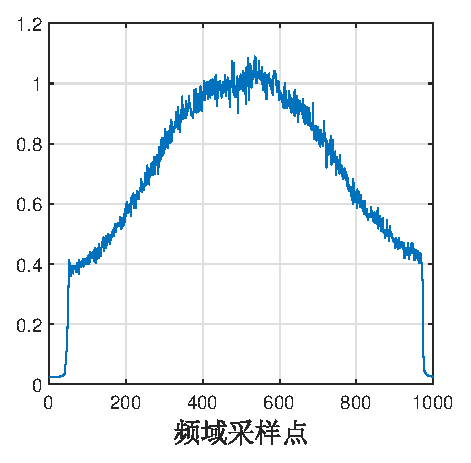
\includegraphics[width=4.cm]{output2/spec1.eps}}
  \subfigure[均衡后的频谱]{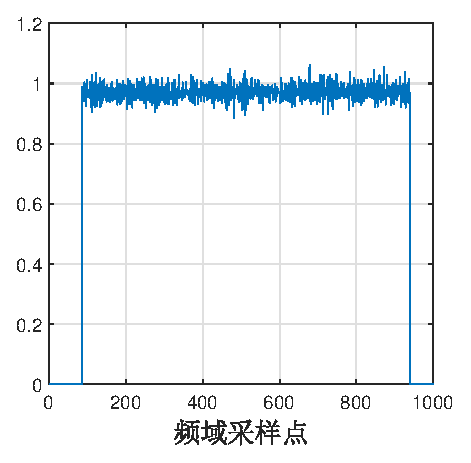
\includegraphics[width=4.cm]{output2/spec1_eq.eps}}
\bicaption{图}{频谱均衡示意图}{Fig.}{Illustration of spectrum equalization}\label{fig:spec-eq}
\end{figure}

\begin{figure}[t]
  \centering
  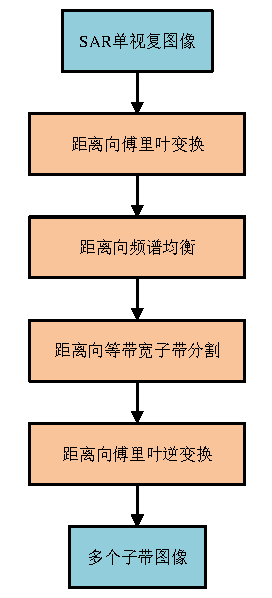
\includegraphics[width=4.3cm]{subband_divide.pdf}
  \bicaption{图}{子带图像生成流程图}{Fig.}{Diagram of subband image generation}\label{fig:subband_divide}
\end{figure}

\subsection{无干扰SAR像素在子带域起伏的几种机制}

SAR成像的点扩展函数近似为二维sinc函数。考虑任意像素点，其对应的网格点坐标用$(R,x)$表示，那么该像素点的值可用如下积分式表示
\begin{equation}\label{eq:pixel-model}
\begin{split}
I(R,x)=\iint &a(x,R) \exp\left(-j4\pi f_0\frac{R}{c}\right)\\
&\cdot \mathrm{sinc}\left(\frac{R-R_0}{\rho_{\rm r}}\right)\mathrm{sinc}\left(\frac{x-x_0}{\rho_{\rm a}}\right)dRdx
\end{split}
\end{equation}
式中，$a(x,R)$表示观测区域在方位-距离平面内的散射系数，$\rho_a$和$\rho_r$分别表示SAR方位和距离分辨率。
简言之，该式说明每一像素值由多个散射点相干叠加得到。
将图像在距离频率维度划分为$N_{\rm s}$个带宽相等的子带。
我们用$f_k$表示第$k$个子带的中心频率，其表达式为
\begin{equation}\label{}
f_k= f_0-\frac{B}{2}+\left(k-\frac{1}{2}\right) \frac{B}{N_{\rm s}}
\end{equation}
子带划分后，不仅中心频率相对于原图像的距离向中心频率发生了变化，距离分辨率也不同：各子带分辨率降低至$N_{\rm s}\rho_{\rm r}$。参照式(\ref{eq:pixel-model})，并考虑散射系数在频带内近似不变，我们可将子带划分后的图像像素表示为
\begin{equation}\label{eq:pixel-model2}
\begin{split}
I_k(R,x)=\iint &a(x,R) \exp\left(-j4\pi f_k\frac{R}{c}\right)\\
&\cdot {\rm \mathrm{sinc}}\left(\frac{R-R_0}{N_{\rm s}\rho_{\rm r}}\right){\rm \mathrm{sinc}}\left(\frac{x-x_0}{\rho_{\rm a}}\right)dRdx
\end{split}
\end{equation}


对于每一像素包含的散射单元成分，我们可分如下几种情况讨论：
\begin{enumerate}
\setlength{\itemsep}{0pt}
\setlength{\parsep}{0pt}
  \item 分辨单元内由许多基本散射点组成，且无主导散射点。这种情况下，SAR图像像素表现为相干斑。不同子带的中心频率$f_k$不同，那么由信号传播引入的相位$\exp\left(-j4\pi f_kR/c\right)$在不同子带中也是不同的，这造成同一分辨单元内不同散射体在不同子带内以不同矢量方向叠加，最终导致同一网格点像素的幅度在不同子带内是不一致的，统计上随机起伏。这种随机起伏可通过多视处理或空域平均降低。
  \item 分辨单元内由少量强度接近的散射点组成。这种情况下，SAR图像像素表现为不完全发育的相干斑。这种情况和完全发育的相干斑情况类似，同一分辨单元内不同散射体在不同子带内以不同矢量方向叠加，造成同一像素的幅度在不同子带内存在起伏。这种起伏可通过多视处理或空域平均降低。但需要指出，在相同的视数或平滑窗处理后，不完全发育的相干斑的起伏高于完全发育的相干斑的起伏。
  \item 分辨单元内只有一个散射点。这种情况下，根据式(\ref{eq:pixel-model})可知由信号传播引入的相位不影响像素幅度，所以同一像素在不同子带内的强度是相同的。但实际中几乎不存在理想点目标。
  \item 分辨单元内由一个强散射点和多个弱点组成。人造散射体往往具有一个强散射点和多个弱散射点组成，这种情况实际中较多。由于存在主导强散射点，这种情况下同一像素在不同子带内的强度是接近的。
\end{enumerate}

根据上述分析，我们可知无干扰的单视复图像的像素强度在子带域的起伏主要是由相干斑造成的。假设相干斑在各像素局部服从相同的复高斯分布，我们可通过用空域$L$个像素强度(即复值像素模的平方)的滑动平均降低相干斑的方差，即抑制相干斑的起伏。这一过程在SAR图像处理中通常被称为多视处理。多视处理后的相干斑像素强度服从Gamma分布，表达式如下
\begin{equation}\label{}
  f(x;\sigma,\tilde{L})=\frac{1}{\Gamma(\tilde{L})}\biggl(\frac{\tilde{L}}{\sigma}\biggr)^{\tilde{L}}  x^{\tilde{L}-1}\exp\left(-\frac{\tilde{L}\, x}{\sigma}\right)
\end{equation}
其中，参数$\tilde{L}$为等效视数，$\sigma$为多视之前复值像素的方差。若相邻各像素服从独立同分布的复高斯分布，则$\tilde{L}$等同于用于平均的像素个数$L$。实际中，过采样(通常为1.1$\sim$1.2左右)使得相邻像素存在一定的相关性，所以像素的独立性不满足。地物散射系数随空域的变化使得相邻像素不满足同分布假设。上述因素使等效视数$\tilde{L}$小于实际视数$L$。等效视数可用矩估计方法获得。基于上述分析，我们将采用多视降低相干斑在子带域的起伏。



\subsection{间歇采样转发干扰在子带域的起伏机制分析}

间歇采样转发干扰在不同子带的分量可用傅里叶变换予以分析。具体来说，被转发的干扰在第$k$个子带的分量可表示为
\begin{equation}
J_k = \int {\rm rect}\left(\frac{f-f_k}{B/N_{\rm s}}\right) \left|S_{\rm j}(f)\right|^2  df
\end{equation}
因为干扰信号频谱$S_{\rm j}(f)$只在部分带宽内非零，所以干扰信号能量在频域是不均匀分布的。因此，上式积分结果随$k$变化，即SAR图像中的干扰分量$J_k$在不同子带中存在起伏。

\begin{figure}[t]
  \centering
  \setcounter{subfigure}{0}
  \subfigure[SAR图像含有一串间歇采 \newline\centerline{样转发干扰}]{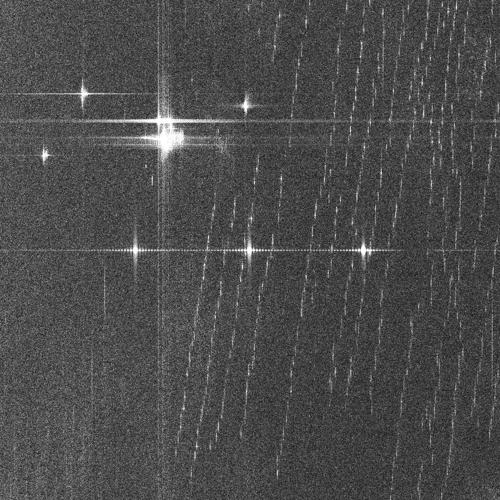
\includegraphics[width=3.7cm,height=3.7cm]{output2/gf3_data1_jam.jpg}}
  \subfigure[干扰在信号域的时频图(横 \newline\centerline{轴：时间，纵轴：频率)}]{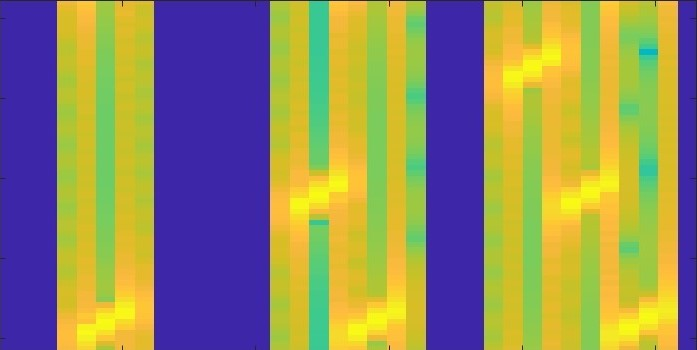
\includegraphics[width=3.7cm,height=3.7cm]{output2/jam_tfd.jpg}}
\bicaption{图}{SAR图像间歇采样转发干扰示例与干扰的时频图}{Fig.}{Example ISRJ in a SAR image and its spectrogram}\label{fig:example}
\end{figure}

为了直观地说明上述目标和干扰在子带域的不同起伏特性，我们进行实例分析。具体而言，我们先在一幅无干扰的高分3号单视复图像中加入仿真的间歇采样循环转发干扰图像，得到含干扰的图像。干扰信号的时频图如图3(b)所示，含干扰的图像如图3(a)所示。仿真涉及的SAR参数如下：载频 5.4GHz，平台速度 7100 m/s，信号带宽 60 MHz，采样率 72 MHz，脉冲重复频率 1800 Hz，场景中心斜距 850 Km，脉冲宽度 50 $\mu$s，斜视角 0 $^{\circ}$，天线长度 10.5 m。然后，我们将该图像按照前述方法划分为10幅子带图像。所得子带图像如图4和图5所示。
观察图5中这10幅子带图，可以发现干扰像素的强度在不同子带中起伏变化，而非干扰区域像素的强度在不同子带中则相对较为稳定。
我们在图4(a)中画出了三组不同像素在子带域的起伏曲线。三组像素分别为干扰像素、强目标像素、背景像素，每组含三个像素。图中P1、P2、P3为强目标像素的起伏曲线，P4、P5、P6为背景像素的起伏曲线，P7、P8、P9为干扰像素的起伏曲线。背景像素是完全发育的相干斑像素，强目标为不完全发育的相干斑像素。可以发现，背景像素幅度起伏最小，强目标像素起伏稍大，干扰像素起伏最大。
图4(b)中显示了方位向多视平均后的子带起伏曲线。与未经多视处理的子带起伏曲线对比，我们发现：多视后的强目标和背景像素的起伏程度变低，而干扰像素的起伏程度则没有变低。

\begin{figure*}
\setcounter{subfigure}{0}
  \centering
  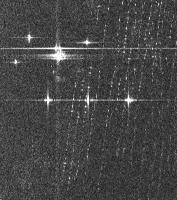
\includegraphics[width=3.3cm,height=3.3cm]{output2/gf3_data1_sublook_1.jpg}
  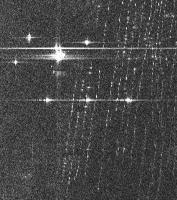
\includegraphics[width=3.3cm,height=3.3cm]{output2/gf3_data1_sublook_2.jpg}
  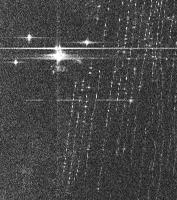
\includegraphics[width=3.3cm,height=3.3cm]{output2/gf3_data1_sublook_3.jpg}
  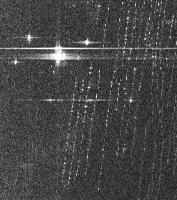
\includegraphics[width=3.3cm,height=3.3cm]{output2/gf3_data1_sublook_4.jpg}
  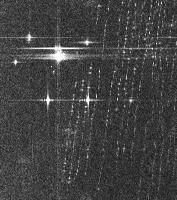
\includegraphics[width=3.3cm,height=3.3cm]{output2/gf3_data1_sublook_5.jpg}\\\vspace{0.08cm}
  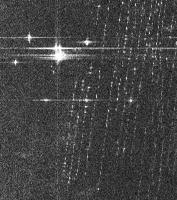
\includegraphics[width=3.3cm,height=3.3cm]{output2/gf3_data1_sublook_6.jpg}
  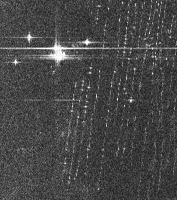
\includegraphics[width=3.3cm,height=3.3cm]{output2/gf3_data1_sublook_7.jpg}
  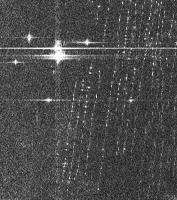
\includegraphics[width=3.3cm,height=3.3cm]{output2/gf3_data1_sublook_8.jpg}
  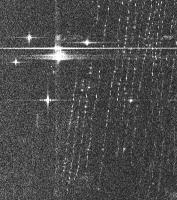
\includegraphics[width=3.3cm,height=3.3cm]{output2/gf3_data1_sublook_9.jpg}
  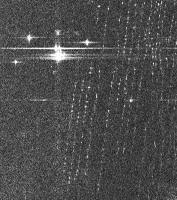
\includegraphics[width=3.3cm,height=3.3cm]{output2/gf3_data1_sublook_10.jpg}
\bicaption{图}{一幅含间歇采样转发干扰的SAR图像所生成的十幅子带图像}{Fig.}{Ten subband images generated from a SAR image having ISRJ}\label{fig:sublook-imgs}
\end{figure*}

上述实例分析表明，干扰像素和非干扰像素在子带域的起伏特性存在显著差异。这一特性可以用来在单视复图像中检测间歇采样转发干扰。






\section{SAR图像子带对比度与子带熵的概念定义与统计分析}

刻画SAR像素子带域起伏程度的统计量的设计对提取干扰特征至关重要。本节给出SAR图像子带对比度和子带熵统计量的概念定义，并分析无干扰情况下二者的统计特性。这两个统计量可以有效描述SAR像素子带域的起伏程度，从而可用于提取干扰区域的特征并用于检测干扰区域。具体的检测流程将在第\ref{sec:dtc}节给出。

\begin{figure}[t]
  \centering
  \setcounter{subfigure}{0}
  \subfigure[子带图未经多视处理]{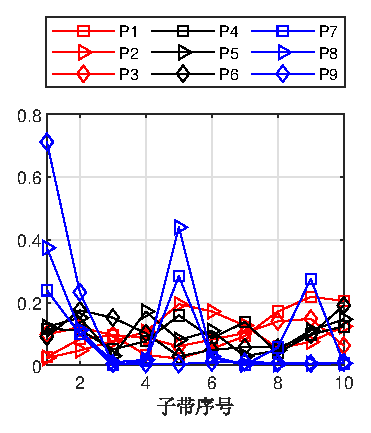
\includegraphics[width=4.cm]{output2/gf3_data1_sublook_profile.eps}}
  \subfigure[子带图在方位向经过多视处理，\newline\centerline{视数为10}]{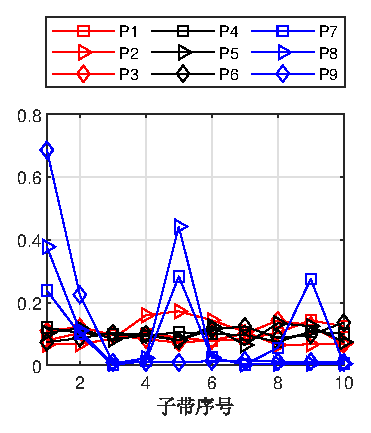
\includegraphics[width=4.cm]{output2/gf3_data1_sublook_profile_ml.eps}}
\bicaption{图}{强目标像素(P1-P3)、背景像素(P4-P6)、干扰像素(P7-P9)的子带域起伏曲线}{Fig.}{The fluctuation profiles of strong pixels (P1-P3), background pixels (P4-P6), and interference pixels (P7-P9)}\label{fig:sublook-profile}
\end{figure}

\subsection{子带对比度}

对比度是在不同学科领域中有特定定义的一个术语，但其核心概念通常涉及到两个或多个元素之间的差异性。在图像处理中，对比度通常是指图像中最亮和最暗部分之间的差异程度。而在SAR信号处理中，对比度则有不同的定义。例如，Yeo等人提出如下对比度定义\upcite{chan1998noniterative}
\begin{equation}
C_l=1-\frac{\left|\frac{1}{T_{\rm aperture}}\int_{-T_{\rm aperture}/2}^{T_{\rm aperture}/2}\lvert\nu_l(\eta)\rvert dt \right|^2}{\frac{1}{T_{\rm aperture}}\int_{-T_{\rm aperture}/2}^{T_{\rm aperture}/2}\lvert\nu_l(\eta)\rvert ^2dt}
\end{equation}
其中，$T_{\rm aperture}$表示合成孔径时长，$\nu_l(\eta)$表示距离压缩后第$l$个距离单元的方位向信号。该式定义的对比度是对主导散射体强度方差的一种度量。在距离压缩相位历史域，理想点目标会在方位向产生较为恒定幅度的信号，导致低对比度。强散射点的方位信号的对比度值通常小于0.1，Yeo等人将这一指标用于选取强散射点的方位信号，并用于SAR相位梯度自聚焦成像。借鉴于这一思想，本文定义如下子带对比度统计量
\begin{equation}\label{eq:C}
C[n,m] = 1-\frac{\left(\frac{1}{N_{\rm s}}\sum_{k=1}^{N_{\rm s}} |I_k[n,m]|\right)^2}{\frac{1}{N_{\rm s}}\sum_{k=1}^{N_{\rm s}}|I_k[n,m]|^2}
\end{equation}
上式中定义的对比度的取值范围是$[0,1-1/N_{\rm s}]$，证明如下。首先证明子带对比度的最小值为0。根据柯西不等式可知$\left(\sum_{k=1}^{N_{\rm s}} |I_k[n,m]|\right)^2\le{{N_{\rm s}}\sum_{k=1}^{N_{\rm s}} |I_k[n,m]|^2}$，当且仅当$|I_1[n,m]|=|I_2[n,m]|,\cdots,|I_{N_{\rm s}}[n,m]|$时等号成立。将此不等式带入式(\ref{eq:C})可得$C\ge 0$，子带对比度的最小值为0。然后，证明子带对比度最大值为$1-1/N_{\rm s}$。我们对上式中分式$\frac{(\frac{1}{N_{\rm s}}\sum_{k=1}^{N_{\rm s}} |I_k[n,m]|)^2}{\frac{1}{N_{\rm s}}\sum_{k=1}^{N_{\rm s}} |I_k[n,m]|^2}$的分子进行展开，可得如下关系
\begin{equation}\label{}
\begin{split}
  &\frac{\left(\frac{1}{N_{\rm s}}\sum_{k=1}^{N_{\rm s}} |I_k[n,m]|\right)^2}{\frac{1}{N_{\rm s}}\sum_{k=1}^{N_{\rm s}} |I_k[n,m]|^2} \\
  &= \frac{1}{N_{\rm s}} + \frac{ 2\sum_{k\neq k'} |I_k[n,m]|\cdot|I_{k'}[n,m]|}{{N_{\rm s}}\sum_{k=1}^{N_{\rm s}} |I_k[n,m]|^2}  \le \frac{1}{N_{\rm s}}
\end{split}
\end{equation}
当且仅当$\{|I_k[n,m]|\,\big| \, k=1,\cdots,N_{\rm s}\}$只有一个非零元素时，不等式的等号成立。将此不等式带入式(\ref{eq:C})可得$C\le 1-\frac{1}{N_{\rm s}}$，子带对比度的最大值为$1-\frac{1}{N_{\rm s}}$。为了便于后续分析，我们将子带对比度进行归一化处理
\begin{equation}\label{}
  \tilde{C}[n,m] = C[n,m]\frac{N_{\rm s}}{N_{\rm s}-1}
\end{equation}
本文后续讨论中的对比度将采用该式所定义的归一化的对比度。


\subsection{子带熵}

熵是用来描述系统的无序程度或信息的不确定性的一种度量。香农提出了信息熵的定义\upcite{shannon1948mathematical}
\begin{equation}\label{eq:E0}
E = -\sum_{k=1}^{N} p_k \log p_k
\end{equation}
其中，$p_k$表示概率。其取值范围是$[0,\log N]$，证明过程如下。
首先分析熵的最小值。由$0\le p_k\le1$可知熵取值非负。当有一个$p_k$取值为1时，其他$p_k$取值为0，这一取值条件下熵值为0。因此，熵最小值为0。然后分析熵的最大值。
由于概率和为1，我们可得等式约束方程$\sum_{k=1}^N p_k = 1$。利用拉格朗日乘子法，将熵$E$的表达式(\ref{eq:E0})与上述概率约束方程用拉格朗日乘子$\mu$组合，得到如下拉格朗日函数
\begin{equation}\label{}
  L(p_1,\cdots,p_{N},\lambda) = -\sum_{k=1}^N p_k \log p_k + \mu (1-\sum_{k=1}^N p_k)
\end{equation}
由于该函数的极大值取值点$(p_1,\cdots,p_{N},\lambda)$满足偏导数为0，我们可得到如下方程组
\begin{equation}\label{}
  \frac{\partial L}{\partial p_k} = -\log p_k  -1 + \mu = 0, \quad k=1,\cdots,N
\end{equation}
显然，根据上式可得熵最大时所有的$p_k$相等。再结合$\sum_{k=1}^N p_k=1$，可得$p_k=1/N$。将$p_k=1/N$带入式(\ref{eq:E0})可得熵最大值为$\log N$。上述熵取值范围与对数的底数有关。
\begin{figure}[t]
\setcounter{subfigure}{0}
  \centering
  \subfigure[子带对比度]{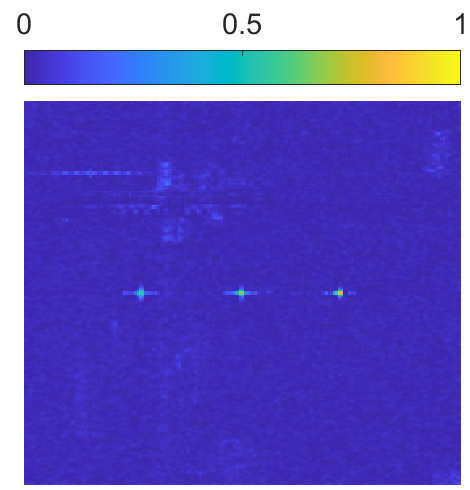
\includegraphics[width=4.cm]{output2/contrast_demo.png}}
   \subfigure[子带熵]{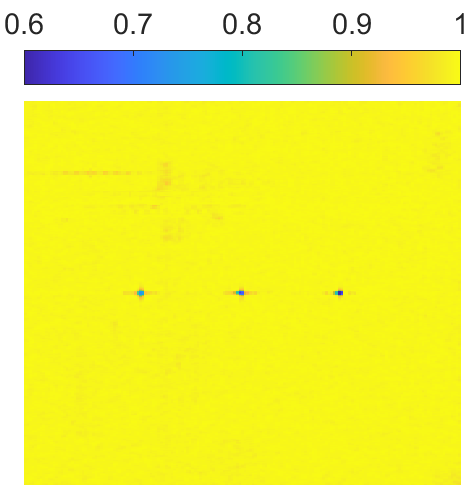
\includegraphics[width=4.cm]{output2/entropy_demo.png}}
  \bicaption{图}{一幅单视复SAR图像计算得到的子带对比度和子带熵示例}{Fig.}{Examples of subband contrast and subband entropy for a SAR image with ISRJ}\label{fig:contrast-entropy}
\end{figure}

在SAR成像算法领域，学者们定义$p_k$为每一像素相对于总图像的能量占比，并借用熵这一概念以描述SAR图像的聚焦程度，从而提出了最小熵自聚焦算法。这一思想可追溯到1990年左右\upcite{bocker1991new}。对比度和熵用于成像算法领域的工作和应用可参见文献\cite{chen2021motion}。此外，熵在极化SAR领域也是一种重要的特征提取与目标识别工具\upcite{yangj2020book}。在本文中，我们定义$p_k[n,m]$为该网格点的子带$k$像素相对于全部子带像素能量之和的占比
\begin{equation}\label{}
  p_k[n,m]=\frac{|I_k[n,m]| ^2}{\sum_{k=1}^{N_{\rm s}} |I_k[n,m]|^2}
\end{equation}
基于此，我们定义如下归一化的子带熵统计量
\begin{equation}
\tilde{E}[n,m] = -\frac{1}{\log N_{\rm s}}\sum_{k=1}^{N_{\rm s}} p_k[n,m] \log p_k[n,m] 
\end{equation}
其取值范围为$[0,1]$，与对数的底数无关。


\subsection{子带对比度和子带熵的统计分析与Beta分布拟合}

\begin{figure*}[t]
\setcounter{subfigure}{0}
  \centering
  \subfigure[数据1]{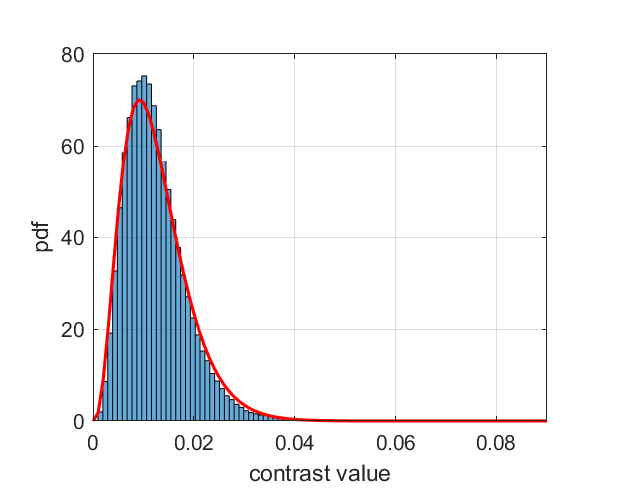
\includegraphics[width=5.3cm]{output2/GF3_FSI/beta_fitting_contrast.eps}}\quad
  \subfigure[数据2]{
\includegraphics[width=5.3cm]{output2/MV3D3/beta_fitting_contrast.eps}}\quad
  \subfigure[数据3]{
\includegraphics[width=5.3cm]{output2/MV3D2/beta_fitting_contrast.eps}}\\
  \subfigure[数据1]{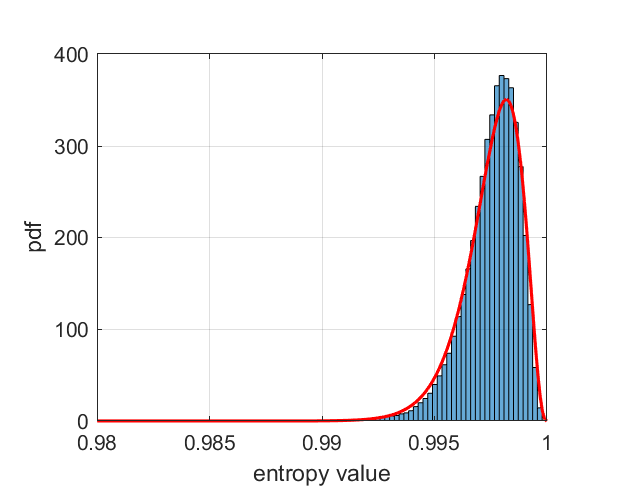
\includegraphics[width=5.3cm]{output2/GF3_FSI/beta_fitting_entropy.eps}}\quad
  \subfigure[数据2]{
\includegraphics[width=5.3cm]{output2/MV3D3/beta_fitting_entropy.eps}}\quad
  \subfigure[数据3]{
\includegraphics[width=5.3cm]{output2/MV3D2/beta_fitting_entropy.eps}}
  \bicaption{图}{子带对比度和子带熵样本的直方图分布和Beta分布概率密度函数拟合结果示例}{Fig.}{Example of histogram distribution and beta fitting results of subband contrast and subband entropy}\label{fig:beta-fitting}
\end{figure*}

\begin{figure*}[t]
\setcounter{subfigure}{0}
  \centering
  \subfigure[数据1]{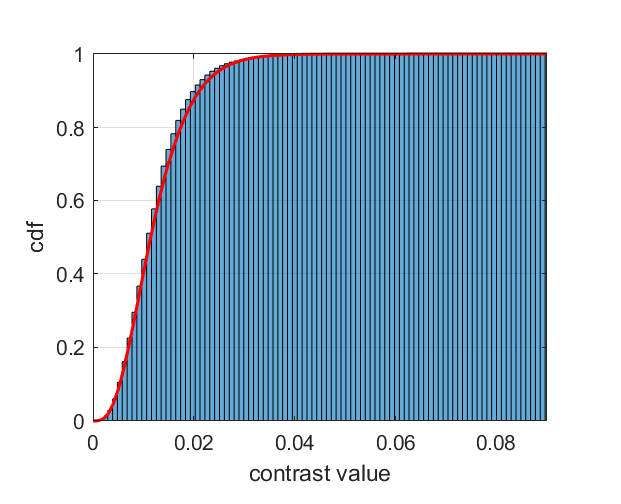
\includegraphics[width=5.3cm]{output2/GF3_FSI/beta_cdf_fitting_contrast.eps}}\quad
  \subfigure[数据2]{
\includegraphics[width=5.3cm]{output2/MV3D3/beta_cdf_fitting_contrast.eps}}\quad
  \subfigure[数据3]{
\includegraphics[width=5.3cm]{output2/MV3D2/beta_cdf_fitting_contrast.eps}}\\
  \subfigure[数据1]{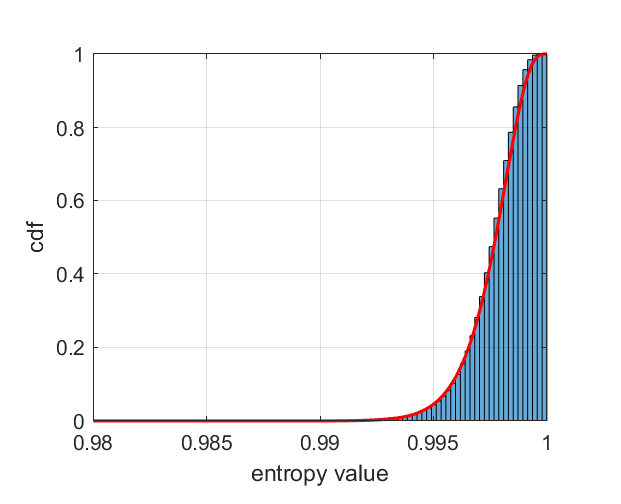
\includegraphics[width=5.3cm]{output2/GF3_FSI/beta_cdf_fitting_entropy.eps}}\quad
  \subfigure[数据2]{
\includegraphics[width=5.3cm]{output2/MV3D3/beta_cdf_fitting_entropy.eps}}\quad
  \subfigure[数据3]{
\includegraphics[width=5.3cm]{output2/MV3D2/beta_cdf_fitting_entropy.eps}}
  \bicaption{图}{子带对比度和子带熵样本的累计直方图分布和Beta分布累计概率密度函数拟合结果示例}{Fig.}{Example of cumulative histogram and beta fitting results for subband contrast and subband entropy}\label{fig:beta-cdf-fitting}
\end{figure*}

上文定义的子带对比度和子带熵的取值都是在0和1之间。从图6可以看出，无干扰像素的子带对比度值小而子带熵值大，且二者取值具有随机性。

我们希望找到某种分布函数以描述无干扰像素的子带对比度和子带熵的这种随机性，从而便于我们以统计学的角度选取检测阈值。为此，我们对真实数据的子带熵和子带对比度进行了直方图分析，因为直方图的包络能够反映出数据的分布。根据真实数据得出的直方图，我们发现子带对比度和子带熵近似服从Beta分布。

Beta分布是随机变量取值在0和1之间的分布，其分布函数的表达式为
\begin{equation}
    f\left(x;\alpha,\beta\right)=\frac1{B\left(\alpha,\beta\right)}x^{\alpha-1}(1-x)^{\beta-1}
\end{equation}
其中，$B(a,b)$为Beta函数，定义式为
\begin{equation}
    B(a,b)=\frac{\Gamma(a)\Gamma(b)}{\Gamma(a+b)}
\end{equation}
其中，$\Gamma(\cdot)$表示Gamma函数。该分布函数含有未知参数$(a,b)$。我们需要获得这两个未知参数，才能用上式分布函数对上述子带对比度和子带熵进行统计分析。为此，我们采用矩估计方法从数据中估计参数$(a,b)$。具体过程如下所述。首先，我们给出Beta分布的均值和方差表达式
\begin{subequations}
\begin{align}
  m & =\frac{a}{a+b} \\
 v &  = \frac{ab}{(a+b+1)^2(a+b)^2}
\end{align}
\end{subequations}
将$(a,b)$视为二元未知量，以$(m,v)$为已知量，那么上式为关于$(a,b)$的二元方程组。利用消元法求$(a,b)$关于$(m,v)$的表达式，可得
\begin{subequations}\label{eq:ab}
\begin{align}
  a &=-\frac{m}{v}(m^2-m+v) \\
  b & =\frac{m}{v}(m-1)^2 + m -1
\end{align}
\end{subequations}
均值和方差可用计算得到的子带对比度或子带熵的均值$\hat{m}$和方差$\hat{v}$作为估计量。以对比度为例，均值和方差的无偏估计分别为
\begin{subequations}
\begin{align}
\hat{m} &=  \frac{1}{N_a N_r}   \sum_{n=1,k=1}^{N_a,N_r} C[n,k] \\
\hat{v} &= \frac{1}{N_a N_r -1} \sum_{n=1,k=1}^{N_a,N_r} |C[n,k]-\hat{m}|^2
\end{align}
\end{subequations}
将这一组估计带入式(\ref{eq:ab})，可得参数$(a,b)$的估计。图7和图8给出了子带对比度和子带熵样本的直方图分布和Beta分布拟合结果示例，其中数据1为高分3号FSI数据，数据2和数据3是SARMV3D数据\upcite{qiu2021sarmv3d}。上述分布拟合结果可用于下文中恒虚警检测阈值的设置。



\section{基于SAR图像子带对比度和子带熵的干扰检测方法}\label{sec:dtc}

本节将给出用子带对比度和子带熵的进行干扰检测的具体方法和详细检测流程。我们还将讨论检测阈值的选取方法，以及将检测结果用于自适应干扰抑制。

\subsection{干扰检测的假设检验模型}

我们将干扰检测问题建模为假设检验问题，含如下一组假设：
\begin{enumerate}
\setlength{\itemsep}{0pt}
\setlength{\parsep}{0pt}
  \item 检验假设${\rm H}_0$：像素$[n,m]$无干扰；
  \item 备择假设${\rm H}_1$：像素$[n,m]$有干扰。
\end{enumerate}
本节将用子带对比度和子带熵作为上述假设检验的统计量。我们先对单视复图像进行子带划分，生成多个子带图像。每个像素网格点$[n,m]$有$N_{\rm s}$个子带像素，我们用$I_k[n,m]$表示。然后，对每一个像素网格点，我们计算其子带对比度$\tilde{C}[n,m]$和子带熵$\tilde{E}[n,m]$。最后，我们将选定的统计量与特定阈值比较以判定该像素网格点是否存在干扰。对于子带对比度，设检测阈值为$\xi_{\rm C}$，如果满足$\tilde{C}[n,m]\ge\xi_{\rm C}$，则判定像素网格点$[n,m]$存在干扰；否则则该像素无干扰。对于子带熵，设检测阈值为$\xi_{\rm E}$，如果满足$\tilde{E}[n,m]\le\xi_{\rm E}$，则判定像素网格点$[n,m]$存在干扰；否则，则该像素无干扰。检测阈值根据恒虚警准则选取，其选取方法在下一小节给出。

\subsection{基于Beta累积分布函数的恒虚警检测阈值选取方法}

上文中我们发现，在无干扰情况下 子带对比度和子带熵统计量的分布接近Beta分布，因此可以在给定虚警概率的条件下用Beta累积分布函数求出检测阈值。Beta分布的累积概率密度函数为
\begin{equation}
  F(x;a,b) = P(X \le x ; {\rm H}_0) = I(x;a,b)=\frac{B_x(a,b)}{B(a,b)}
\end{equation}
式中$I_x(a,b)$ 为正则不完全Beta函数。
\begin{equation}
    B_x(a,b)=\int_0^xt^{a-1}(1-t)^{b-1}dt
\end{equation}
用恒虚警准则进行检测，令随机变量$X$指代无干扰情况下任意待检测像素网格点$[n,m]$的子带对比度，检测阈值为$\xi$，虚警概率为$p_{\rm fa} =P(X\ge \xi ; {\rm H}_0)$，那么可根据该累积概率密度函数求出检测阈值，其表达式为
\begin{equation}
\begin{split}
    \xi&=\big\{\xi:F(\xi;a,b)=1-p_{\rm fa}\big\} = I^{-1}(1-p_{\rm fa} ; a,b)
\end{split}
\end{equation}
其中，$I^{-1}(z;a,b)$为正则不完全Beta函数的逆函数。该逆函数无解析式，其函数值需要通过数值计算获得。很多软件提供了此逆函数的计算功能，例如Python科学计算库scipy提供的betaincinv函数\footnote{\noindent\url{https://docs.scipy.org/doc/scipy/reference/generated/scipy.special.betainc.html}}和MATLAB提供betainv函数\footnote{\noindent\url{https://ww2.mathworks.cn/help/stats/betainv.html}}。

我们需要指出，通常情况下SAR图像中的完全发育或接近完全发育的相干斑像素占绝大多数，所以根据上述方法求出的阈值可控制这类像素的虚警率近似不超过指定的数值。
但实际中存在少数不完全发育的相干斑像素，这类像素的子带域起伏稍大，容易造成虚警，故而需要设置稍高的阈值。本文中，子带对比度阈值取0.2，子带熵阈值取0.95。

\begin{figure}[t]
  \centering
  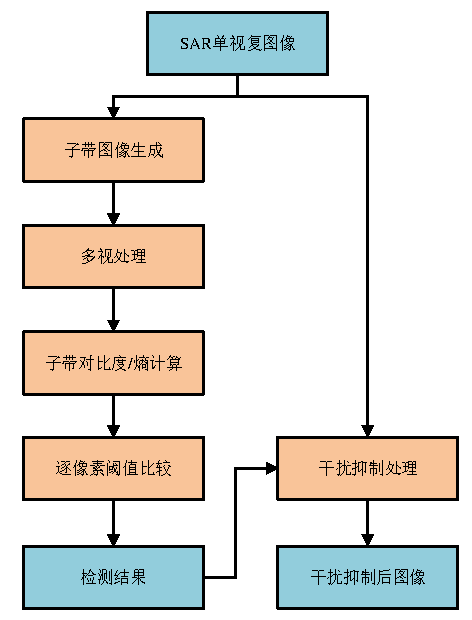
\includegraphics[width=7.cm]{detection_bsf.pdf}
  \bicaption{图}{基于子带对比度/熵的干扰检测与自适应干扰抑制流程}{Fig.}{Interference detection and adaptive interference suppression flow based on subband contrast/entropy}\label{fig:detection_bsf}
\end{figure}

根据上述讨论，我们把干扰检测流程给出在图9所示流程图的左侧支路中。此流程图的右侧支路将干扰检测结果用于自适应干扰抑制，其对应的具体的干扰抑制方法将在第\ref{sec:dtc}.\ref{sec:pca}节给出。

\begin{figure*}[t]
\setcounter{subfigure}{0}
  \centering
  %
\includegraphics[width=3.2cm,height=3.2cm]{output2/e11/img0.jpg}
     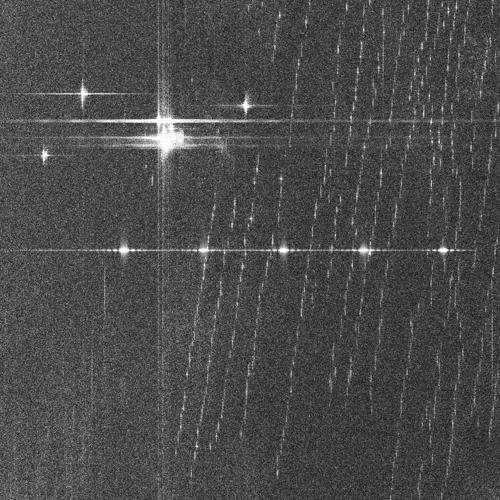
\includegraphics[width=3.2cm,height=3.2cm]{output2/e13/img1.jpg}
      
\includegraphics[width=3.2cm,height=3.2cm]{output2/e13/dt_result_c.jpg}
       
\includegraphics[width=3.2cm,height=3.2cm]{output2/e13/dt_result_e.jpg}
         
\includegraphics[width=3.2cm,height=3.2cm]{output2/e13/img_flt_c.jpg}
          
\includegraphics[width=3.2cm,height=3.2cm]{output2/e13/img_flt_e.jpg}\\     \vspace{0.08cm} 
    
\includegraphics[width=3.2cm,height=3.2cm]{output2/e14/img1.jpg}
      
\includegraphics[width=3.2cm,height=3.2cm]{output2/e14/dt_result_c.jpg}
       
\includegraphics[width=3.2cm,height=3.2cm]{output2/e14/dt_result_e.jpg}
         
\includegraphics[width=3.2cm,height=3.2cm]{output2/e14/img_flt_c.jpg}
          
\includegraphics[width=3.2cm,height=3.2cm]{output2/e14/img_flt_e.jpg}\\    \vspace{0.08cm} 
   
\includegraphics[width=3.2cm,height=3.2cm]{output2/e15/img1.jpg}
      
\includegraphics[width=3.2cm,height=3.2cm]{output2/e15/dt_result_c.jpg}
       
\includegraphics[width=3.2cm,height=3.2cm]{output2/e15/dt_result_e.jpg}
         
\includegraphics[width=3.2cm,height=3.2cm]{output2/e15/img_flt_c.jpg}
          
\includegraphics[width=3.2cm,height=3.2cm]{output2/e15/img_flt_e.jpg}\\  \vspace{-0.09cm} 
    \subfigure[含干扰图像]{
\includegraphics[width=3.2cm,height=3.2cm]{output2/e16/img1.jpg}}
      \subfigure[子带对比度的检测结果]{
\includegraphics[width=3.2cm,height=3.2cm]{output2/e16/dt_result_c.jpg}}
       \subfigure[子带熵的检测结果]{
\includegraphics[width=3.2cm,height=3.2cm]{output2/e16/dt_result_e.jpg}}
         \subfigure[用子带对比度检测并用秩1估计方法去除干扰的结\newline\centerline{果}]{
\includegraphics[width=3.2cm,height=3.2cm]{output2/e16/img_flt_c.jpg}}
          \subfigure[用子带熵检测并用秩1\newline\centerline{估计方法去除干扰的结果}]{
\includegraphics[width=3.2cm,height=3.2cm]{output2/e16/img_flt_e.jpg}}
\bicaption{图}{第一组实验的四种干扰情况和检测与抑制结果}{Fig.}{Four interference conditions and detection and suppression results of the first group of experiments}\label{fig:e1}
\end{figure*}


\begin{figure*}[t]
\setcounter{subfigure}{0}
  \centering
  %
\includegraphics[width=3.2cm,height=3.2cm]{output2/e11/img0.jpg}
     
\includegraphics[width=3.2cm,height=3.2cm]{output2/e23/img1.jpg}
      
\includegraphics[width=3.2cm,height=3.2cm]{output2/e23/dt_result_c.jpg}
       
\includegraphics[width=3.2cm,height=3.2cm]{output2/e23/dt_result_e.jpg}
         
\includegraphics[width=3.2cm,height=3.2cm]{output2/e23/img_flt_c.jpg}
          
\includegraphics[width=3.2cm,height=3.2cm]{output2/e23/img_flt_e.jpg}\\     \vspace{0.08cm} 
    
\includegraphics[width=3.2cm,height=3.2cm]{output2/e24/img1.jpg}
      
\includegraphics[width=3.2cm,height=3.2cm]{output2/e24/dt_result_c.jpg}
       
\includegraphics[width=3.2cm,height=3.2cm]{output2/e24/dt_result_e.jpg}
         
\includegraphics[width=3.2cm,height=3.2cm]{output2/e24/img_flt_c.jpg}
          
\includegraphics[width=3.2cm,height=3.2cm]{output2/e24/img_flt_e.jpg}\\    \vspace{0.08cm} 
   
\includegraphics[width=3.2cm,height=3.2cm]{output2/e25/img1.jpg}
      
\includegraphics[width=3.2cm,height=3.2cm]{output2/e25/dt_result_c.jpg}
       
\includegraphics[width=3.2cm,height=3.2cm]{output2/e25/dt_result_e.jpg}
         
\includegraphics[width=3.2cm,height=3.2cm]{output2/e25/img_flt_c.jpg}
          
\includegraphics[width=3.2cm,height=3.2cm]{output2/e25/img_flt_e.jpg}\\  \vspace{-0.09cm} 
    \subfigure[含干扰图像]{
\includegraphics[width=3.2cm,height=3.2cm]{output2/e26/img1.jpg}}
      \subfigure[子带对比度的检测结果]{
\includegraphics[width=3.2cm,height=3.2cm]{output2/e26/dt_result_c.jpg}}
       \subfigure[子带熵的检测结果]{
\includegraphics[width=3.2cm,height=3.2cm]{output2/e26/dt_result_e.jpg}}
         \subfigure[用子带对比度检测并用秩1估计方法去除干扰的结\newline\centerline{果}]{
\includegraphics[width=3.2cm,height=3.2cm]{output2/e26/img_flt_c.jpg}}
          \subfigure[用子带熵检测并用秩1\newline\centerline{估计方法去除干扰的结果}]{
\includegraphics[width=3.2cm,height=3.2cm]{output2/e26/img_flt_e.jpg}}
\bicaption{图}{第二组实验的四种干扰情况和检测与抑制结果}{Fig.}{Four interference conditions and detection and suppression results of the second group of experiments}\label{fig:e2}
\end{figure*}



\begin{figure*}[t]
  \centering\setcounter{subfigure}{0}
  %
\includegraphics[width=3.2cm,height=3.2cm]{output2/e11/img0.jpg}
     
\includegraphics[width=3.2cm,height=3.2cm]{output2/e33/img1.jpg}
      
\includegraphics[width=3.2cm,height=3.2cm]{output2/e33/dt_result_c.jpg}
       
\includegraphics[width=3.2cm,height=3.2cm]{output2/e33/dt_result_e.jpg}
         
\includegraphics[width=3.2cm,height=3.2cm]{output2/e33/img_flt_c.jpg}
          
\includegraphics[width=3.2cm,height=3.2cm]{output2/e33/img_flt_e.jpg}\\     \vspace{0.08cm} 
    
\includegraphics[width=3.2cm,height=3.2cm]{output2/e34/img1.jpg}
      
\includegraphics[width=3.2cm,height=3.2cm]{output2/e34/dt_result_c.jpg}
       
\includegraphics[width=3.2cm,height=3.2cm]{output2/e34/dt_result_e.jpg}
         
\includegraphics[width=3.2cm,height=3.2cm]{output2/e34/img_flt_c.jpg}
          
\includegraphics[width=3.2cm,height=3.2cm]{output2/e34/img_flt_e.jpg}\\    \vspace{0.08cm} 
   
\includegraphics[width=3.2cm,height=3.2cm]{output2/e35/img1.jpg}
      
\includegraphics[width=3.2cm,height=3.2cm]{output2/e35/dt_result_c.jpg}
       
\includegraphics[width=3.2cm,height=3.2cm]{output2/e35/dt_result_e.jpg}
         
\includegraphics[width=3.2cm,height=3.2cm]{output2/e35/img_flt_c.jpg}
          
\includegraphics[width=3.2cm,height=3.2cm]{output2/e35/img_flt_e.jpg}\\  \vspace{-0.09cm} 
    \subfigure[含干扰图像]{
\includegraphics[width=3.2cm,height=3.2cm]{output2/e36/img1.jpg}}
      \subfigure[子带对比度的检测结果]{
\includegraphics[width=3.2cm,height=3.2cm]{output2/e36/dt_result_c.jpg}}
       \subfigure[子带熵的检测结果]{
\includegraphics[width=3.2cm,height=3.2cm]{output2/e36/dt_result_e.jpg}}
         \subfigure[用子带对比度检测并用秩1估计方法去除干扰的结\newline\centerline{果}]{
\includegraphics[width=3.2cm,height=3.2cm]{output2/e36/img_flt_c.jpg}}
          \subfigure[用子带熵检测并用秩1\newline\centerline{估计方法去除干扰的结果}]{
\includegraphics[width=3.2cm,height=3.2cm]{output2/e36/img_flt_e.jpg}}
\bicaption{图}{第三组实验的四种干扰情况和检测与抑制结果}{Fig.}{Four interference conditions and detection and suppression results of the third group of experiments}\label{fig:e3}
\end{figure*}


\begin{figure*}[!t]
  \centering\setcounter{subfigure}{0}
     
\includegraphics[width=3.2cm,height=3.2cm]{output2/e6/img0.jpg}
      
\includegraphics[width=3.2cm,height=3.2cm]{output2/e6/dt_result_c.jpg}
       
\includegraphics[width=3.2cm,height=3.2cm]{output2/e6/dt_result_e.jpg}
         
\includegraphics[width=3.2cm,height=3.2cm]{output2/e6/img_flt_c.jpg}
          
\includegraphics[width=3.2cm,height=3.2cm]{output2/e6/img_flt_e.jpg}\\   \vspace{0.08cm} 
               
\includegraphics[width=3.2cm,height=3.2cm]{output2/e4/img0.jpg}
      
\includegraphics[width=3.2cm,height=3.2cm]{output2/e4/dt_result_c.jpg}
       
\includegraphics[width=3.2cm,height=3.2cm]{output2/e4/dt_result_e.jpg}
         
\includegraphics[width=3.2cm,height=3.2cm]{output2/e4/img_flt_c.jpg}
          
\includegraphics[width=3.2cm,height=3.2cm]{output2/e4/img_flt_e.jpg}\\
                    \vspace{0.08cm} 
                                
\includegraphics[width=3.2cm,height=3.2cm]{output2/e5/img0.jpg}
      
\includegraphics[width=3.2cm,height=3.2cm]{output2/e5/dt_result_c.jpg}
       
\includegraphics[width=3.2cm,height=3.2cm]{output2/e5/dt_result_e.jpg}
         
\includegraphics[width=3.2cm,height=3.2cm]{output2/e5/img_flt_c.jpg}
          
\includegraphics[width=3.2cm,height=3.2cm]{output2/e5/img_flt_e.jpg}\\
                    \vspace{0.08cm} 
                                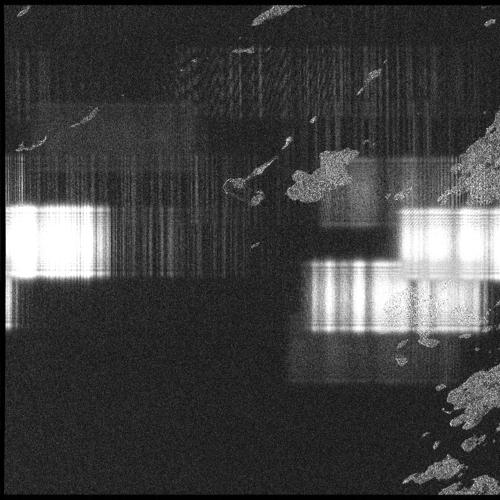
\includegraphics[width=3.2cm,height=3.2cm]{output2/e10/img0.jpg}
      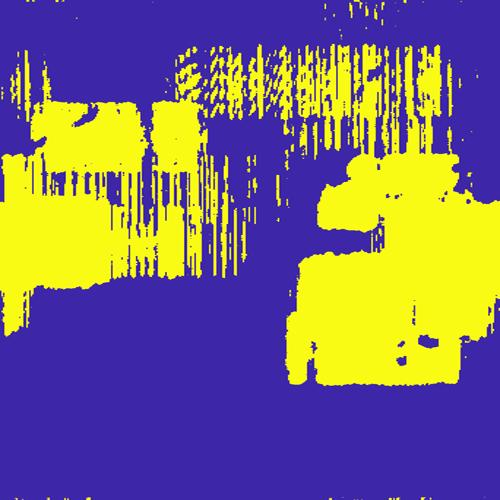
\includegraphics[width=3.2cm,height=3.2cm]{output2/e10/dt_result_c.jpg}
       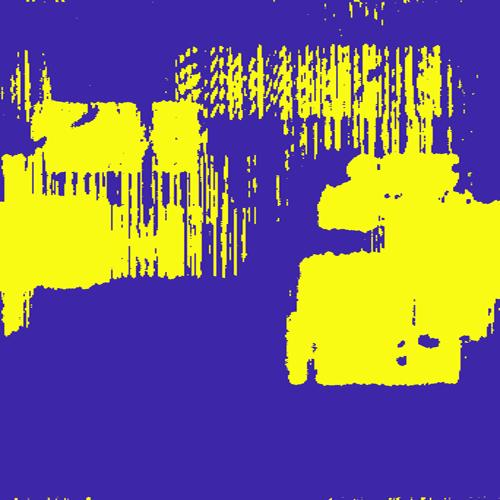
\includegraphics[width=3.2cm,height=3.2cm]{output2/e10/dt_result_e.jpg}
         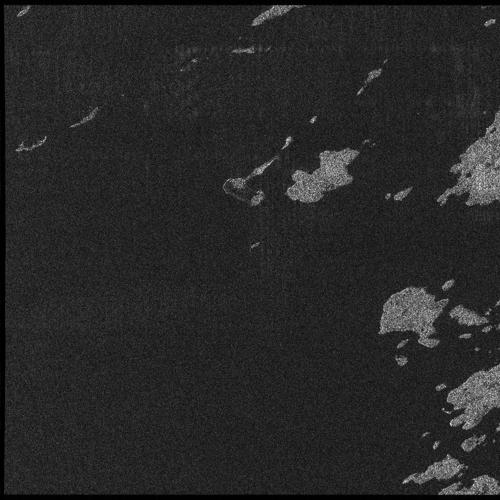
\includegraphics[width=3.2cm,height=3.2cm]{output2/e10/img_flt_c.jpg}
          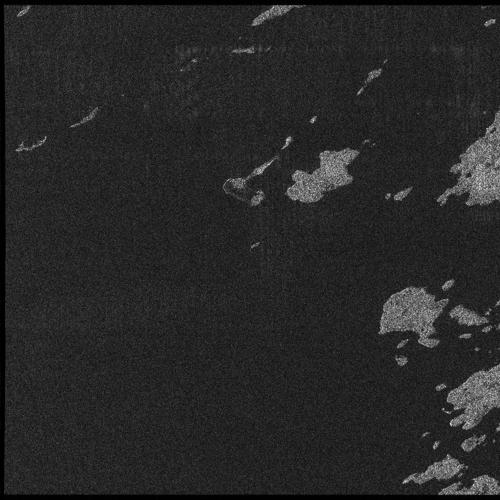
\includegraphics[width=3.2cm,height=3.2cm]{output2/e10/img_flt_e.jpg}\\
                    \vspace{0.08cm} 
               
\includegraphics[width=3.2cm,height=3.2cm]{output2/e7/img0.jpg}
      
\includegraphics[width=3.2cm,height=3.2cm]{output2/e7/dt_result_c.jpg}
       
\includegraphics[width=3.2cm,height=3.2cm]{output2/e7/dt_result_e.jpg}
         
\includegraphics[width=3.2cm,height=3.2cm]{output2/e7/img_flt_c.jpg}
          
\includegraphics[width=3.2cm,height=3.2cm]{output2/e7/img_flt_e.jpg}\\
      \vspace{-0.09cm} 
               \subfigure[含干扰图像]{
\includegraphics[width=3.2cm,height=3.2cm]{output2/e8/img0.jpg}}
\subfigure[子带对比度的检测结果]{
\includegraphics[width=3.2cm,height=3.2cm]{output2/e8/dt_result_c.jpg}}
\subfigure[子带熵的检测结果]{
\includegraphics[width=3.2cm,height=3.2cm]{output2/e8/dt_result_e.jpg}}
\subfigure[用子带对比度检测并去\newline\centerline{除干扰的结果}]{
\includegraphics[width=3.2cm,height=3.2cm]{output2/e8/img_flt_c.jpg}}
          \subfigure[用子带熵检测并去除干\newline\centerline{扰的结果}]{
\includegraphics[width=3.2cm,height=3.2cm]{output2/e8/img_flt_e.jpg}}\\   
\bicaption{图}{第四组实验的干扰检测与抑制结果}{Fig.}{Four interference conditions and detection and suppression results of the fourth group of experiments}\label{fig:e4}
\end{figure*}


\begin{figure*}[t]
  \centering\setcounter{subfigure}{0}
     
\includegraphics[width=2.7cm,height=2.7cm]{output2/e6/img0.jpg}
      
\includegraphics[width=2.7cm,height=2.7cm]{output2/e4/img0.jpg}
       
\includegraphics[width=2.7cm,height=2.7cm]{output2/e5/img0.jpg}
         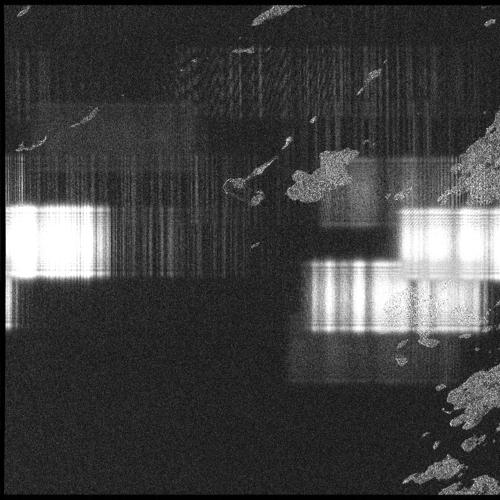
\includegraphics[width=2.7cm,height=2.7cm]{output2/e10/img0.jpg}
          
\includegraphics[width=2.7cm,height=2.7cm]{output2/e7/img0.jpg}
          
\includegraphics[width=2.7cm,height=2.7cm]{output2/e8/img0.jpg}\\   \vspace{0.08cm} 
               
\includegraphics[width=2.7cm,height=2.7cm]{output2/e6/c.jpg}
      
\includegraphics[width=2.7cm,height=2.7cm]{output2/e4/c.jpg}
       
\includegraphics[width=2.7cm,height=2.7cm]{output2/e5/c.jpg}
         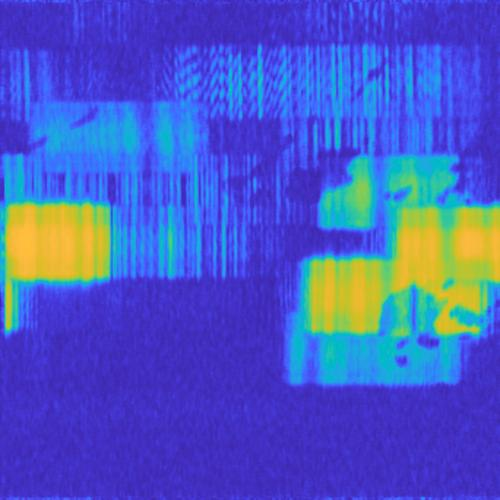
\includegraphics[width=2.7cm,height=2.7cm]{output2/e10/c.jpg}
          
\includegraphics[width=2.7cm,height=2.7cm]{output2/e7/c.jpg}
           
\includegraphics[width=2.7cm,height=2.7cm]{output2/e8/c.jpg}\\  \vspace{0.08cm} 
      
\includegraphics[width=2.7cm,height=2.7cm]{output2/e6/e.jpg}
        
\includegraphics[width=2.7cm,height=2.7cm]{output2/e4/e.jpg}
        
\includegraphics[width=2.7cm,height=2.7cm]{output2/e5/e.jpg}
          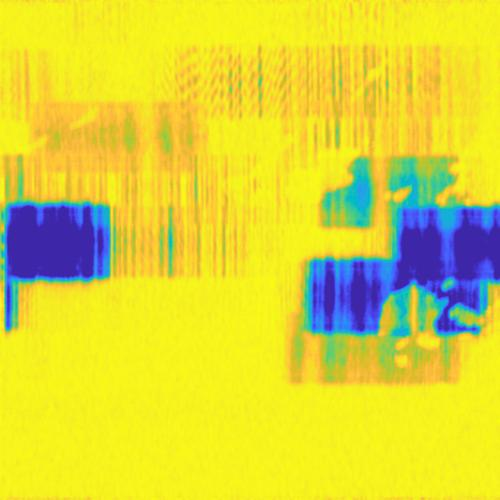
\includegraphics[width=2.7cm,height=2.7cm]{output2/e10/e.jpg}
           
\includegraphics[width=2.7cm,height=2.7cm]{output2/e7/e.jpg}
            
\includegraphics[width=2.7cm,height=2.7cm]{output2/e8/e.jpg}\\    
\bicaption{图}{第四组实验中无意干扰的子带对比度特征图(第二行)和子带熵特征图(第三行)}{Fig.}{Subband contrast feature maps (row 2) and subband entropy feature maps (row 3) in the fourth group of experiments}\label{fig:subbandce}
\end{figure*} 

\begin{figure*}[t]
  \centering\setcounter{subfigure}{0}
  %
\includegraphics[width=3.2cm,height=3.2cm]{output2/e11/img0.jpg}
     \subfigure[第一组干扰像素的子带对比度随JSR的变\newline\centerline{化曲线}]{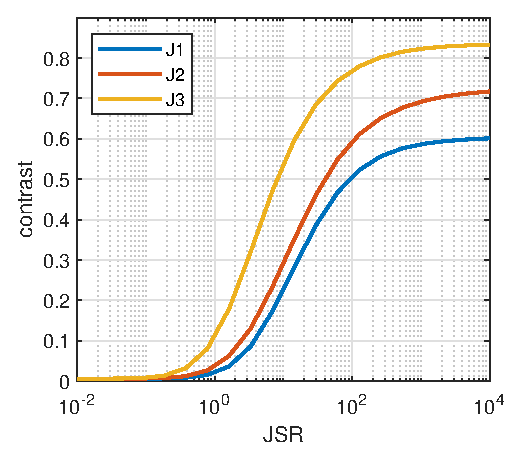
\includegraphics[width=5.3cm]{output2/ce_jsr/c1.eps}}\hspace{0.3cm}
      \subfigure[第一组干扰像素的子带熵随JSR的变化\newline\centerline{曲线}]{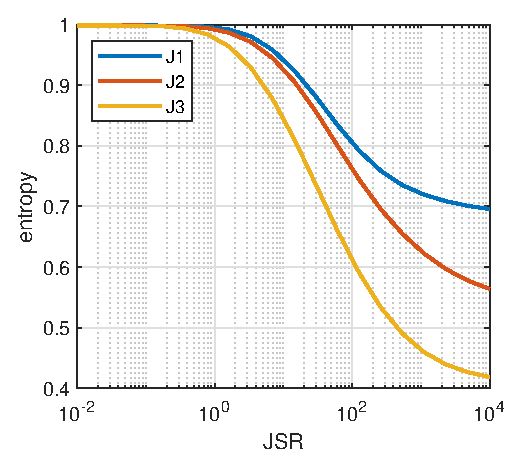
\includegraphics[width=5.3cm]{output2/ce_jsr/e1.eps}}\\
       \subfigure[第二组干扰像素的子带对比度随JSR的变\newline\centerline{化曲线}]{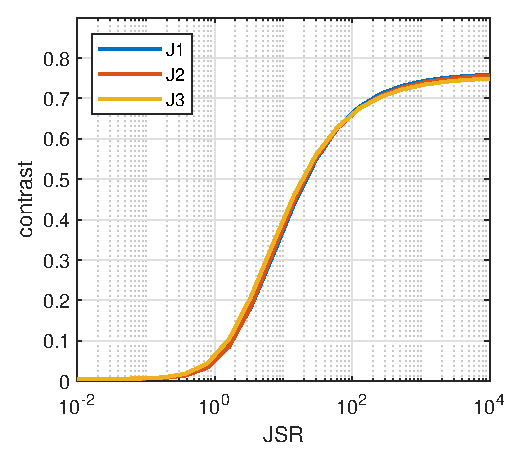
\includegraphics[width=5.3cm]{output2/ce_jsr/c3.eps}}\hspace{0.3cm}
        \subfigure[第二组干扰像素的子带熵随JSR的变化\newline \centerline{曲线}]{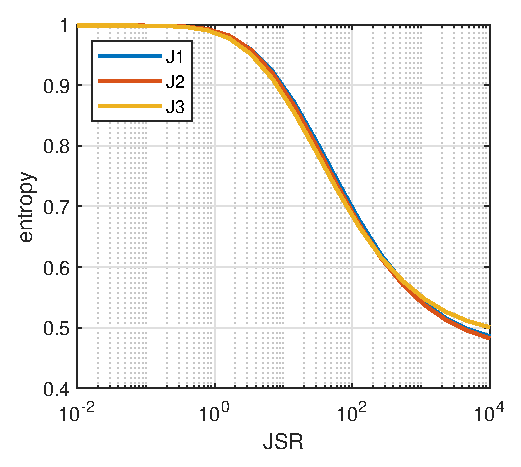
\includegraphics[width=5.3cm]{output2/ce_jsr/e3.eps}}
\bicaption{图}{两组干扰像素的子带对比度和子带熵随JSR的变化曲线}{Fig.}{Curves of subband contrast and subband entropy for two groups of interfering pixels with JSR}\label{fig:ce-jsr}
\end{figure*}


\begin{figure*}[t]
  \centering\setcounter{subfigure}{0}
  %
\includegraphics[width=3.2cm,height=3.2cm]{output2/e11/img0.jpg}
   %\subfigure[pfa, contrast]{\includegraphics[width=5.3cm]{output2/ce_jsr/p/contrast_pfa1.eps}}
  \subfigure[检测概率-子带对比度阈值, JSR=0.5]{\includegraphics[width=5.3cm]{output2/ce_jsr/p/contrast_pd1_jsr_0.5.eps}}
  \subfigure[检测概率-子带对比度阈值, JSR=1]{\includegraphics[width=5.3cm]{output2/ce_jsr/p/contrast_pd1_jsr_1.eps}}
   \subfigure[检测概率-子带对比度阈值, JSR=2]{\includegraphics[width=5.3cm]{output2/ce_jsr/p/contrast_pd1_jsr_2.eps}}\\
  \subfigure[检测概率-虚警概率, JSR=0.5]{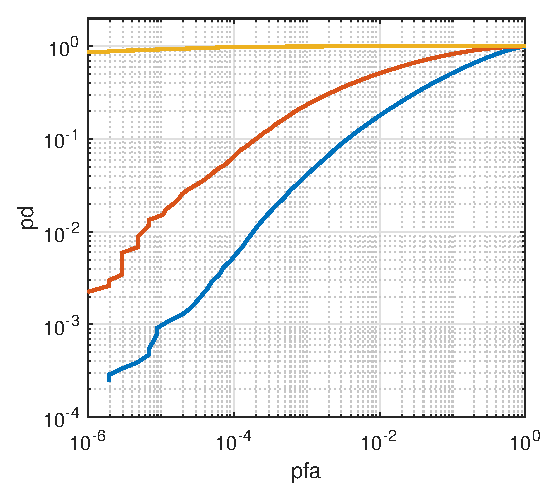
\includegraphics[width=5.3cm]{output2/ce_jsr/p/contrast_pfa_pd1_jsr_0.5.eps}}
   \subfigure[检测概率-虚警概率, JSR=1]{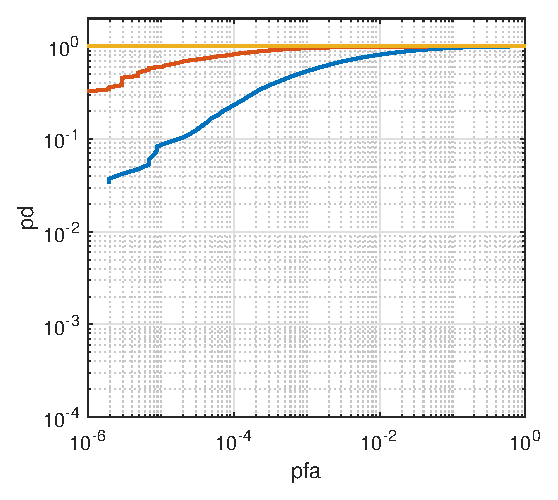
\includegraphics[width=5.3cm]{output2/ce_jsr/p/contrast_pfa_pd1_jsr_1.eps}}
   \subfigure[检测概率-虚警概率, JSR=2]{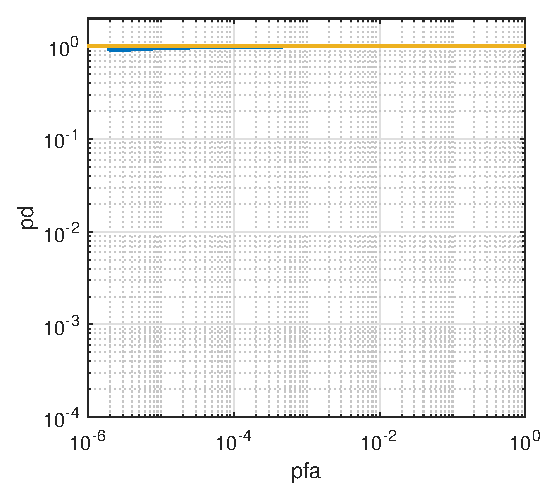
\includegraphics[width=5.3cm]{output2/ce_jsr/p/contrast_pfa_pd1_jsr_2.eps}}
\bicaption{图}{用子带对比度进行检测获得的检测概率随阈值和虚警概率的变化曲线}{Fig.}{Curves of detection probability obtained by detection using subband contrast under different thresholds and false alarm probabilities}\label{fig:p-c}
\end{figure*}


\begin{figure*}[t]
  \centering\setcounter{subfigure}{0}
  %
\includegraphics[width=3.2cm,height=3.2cm]{output2/e11/img0.jpg}
   %\subfigure[pfa, contrast]{\includegraphics[width=5.3cm]{output2/ce_jsr/p/contrast_pfa1.eps}}
  \subfigure[检测概率-子带熵阈值, JSR=0.5]{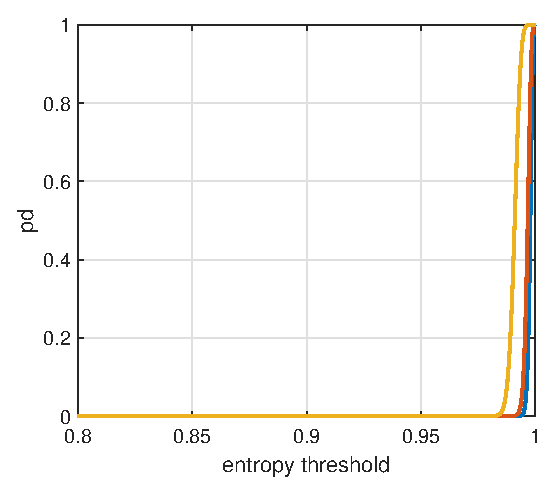
\includegraphics[width=5.3cm]{output2/ce_jsr/p/entropy_pd1_jsr_0.5.eps}}
  \subfigure[检测概率-子带熵阈值, JSR=1]{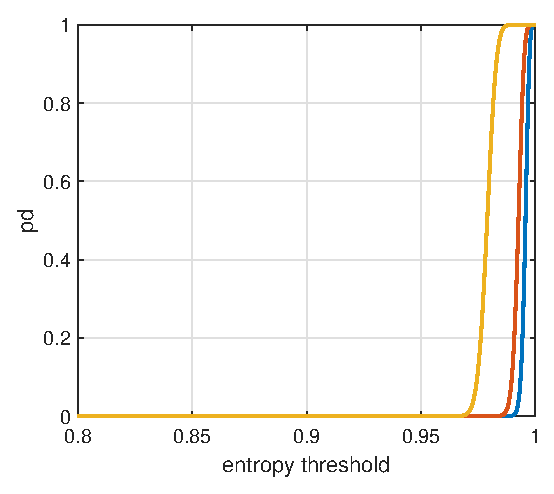
\includegraphics[width=5.3cm]{output2/ce_jsr/p/entropy_pd1_jsr_1.eps}}
   \subfigure[检测概率-子带熵阈值, JSR=2]{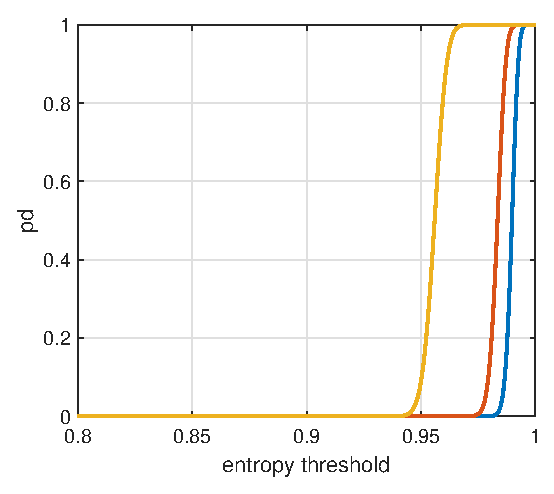
\includegraphics[width=5.3cm]{output2/ce_jsr/p/entropy_pd1_jsr_2.eps}}\\
  \subfigure[检测概率-虚警概率, JSR=0.5]{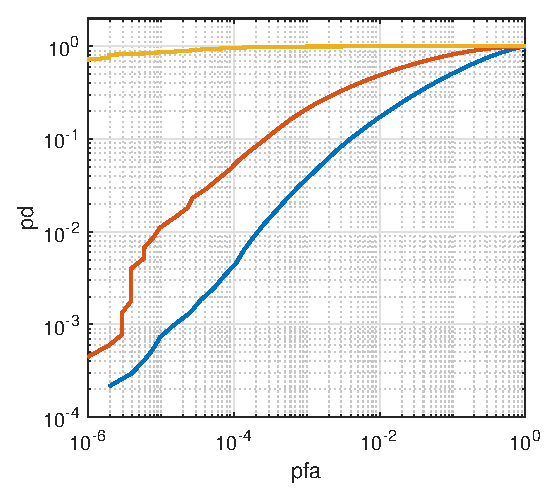
\includegraphics[width=5.3cm]{output2/ce_jsr/p/entropy_pfa_pd1_jsr_0.5.eps}}
   \subfigure[检测概率-虚警概率, JSR=1]{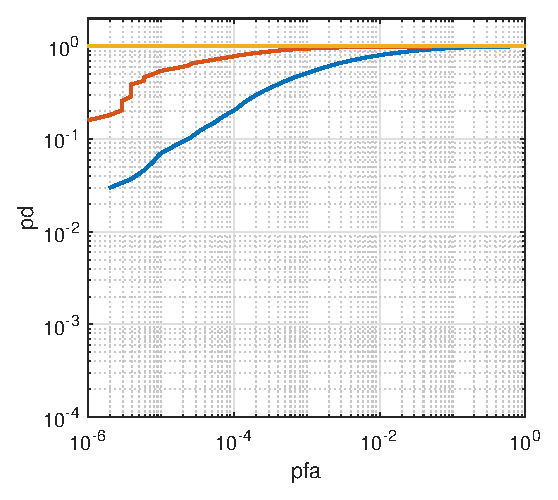
\includegraphics[width=5.3cm]{output2/ce_jsr/p/entropy_pfa_pd1_jsr_1.eps}}
   \subfigure[检测概率-虚警概率, JSR=2]{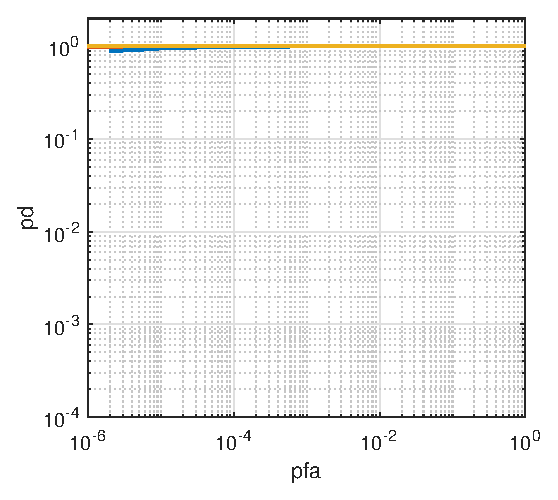
\includegraphics[width=5.3cm]{output2/ce_jsr/p/entropy_pfa_pd1_jsr_2.eps}}
  \bicaption{图}{用子带熵进行检测获得的检测概率随检测阈值和虚警概率的变化曲线}{Fig.}{Curves of detection probability obtained by detection using subband entropy under different thresholds and false alarm probabilities}\label{fig:p-e}
\end{figure*}

\subsection{基于子带对比度/熵检测器与秩1模型的自适应干扰抑制方法}\label{sec:pca}

为了降低干扰对下游任务(例如，目标识别、分类)的影响，我们需要对检测到有干扰的像素区域进行滤波抑制处理。为比，本文采用如下干扰抑制处理流程：

第一步，用上文方法进行干扰检测，得到每个像素的检测结果。该检测结果可用一个二值矩阵$\bf D$表示，矩阵尺寸与原图像相同，值1表示该像素有干扰，值0表示该像素无干扰。

第二步，截取被检测到含干扰的像素与其邻近的若干像素。这些像素作为一个整体可用矩阵$\mathbf{I}_{\rm masked}$在图像域表示。其尺寸与原图像$\mathbf{I}$相同，但是只有被选取的像素区域有值，未被选取的区域置0。该矩阵可用如下式子描述
\begin{equation}
\mathbf{I}_{\rm masked} = (\mathbf{D}*\mathbf{1}_{L_1\times L2}\,>\,0)\circ \mathbf{I}
\end{equation}
其中，$*$表示二维卷积并取卷积结果中与$\mathbf{D}$尺寸相同的中间部分数据，$\mathbf{1}_{L_1\times L_2}$表示尺寸为$L_1\times L_2$且值全为1的矩阵，$>$表示按矩阵元素进行比较的逻辑运算，$\circ$表示两矩阵逐元素相乘运算。


第三步，用秩$1$约束下的最佳F范数逼近以估计并去除干扰成分。间歇采样转发干扰在图像中表现为一串假目标，记为$J(t,\eta)$。其在复数图像域满足如下性质
\begin{equation}\label{eq:uv}
J(t,\eta) \approx \sum_{q=1}^{N_{\rm rank}} u_q(t) v_q(\eta)
\end{equation}
即干扰在复数图像域的成分可表示为若干距离和方位向不耦合的信号之积。举例而言，被转发的脉冲切片在复数图像中的响应近似为若干二维sinc响应的叠加
\begin{equation}\label{eq:isrj-resp}
\begin{split}
J(t,\eta)=
\sum_l &a_l \exp\left(j2\pi \Delta f_{{\rm j},l} t\right)\\
&\cdot{\rm \mathrm{sinc}}\left(\frac{t-t_{{\rm j},l}}{N_{\rm s}\rho_{\rm r}}\right) {\rm \mathrm{sinc}}\left(\frac{\eta-\eta_{{\rm j}}}{\rho_{\rm a}}\right)
\end{split}
\end{equation}
其中，$a_l$表示第$l$个被转发的脉冲切片造成的干扰幅度和相位。$t_{{\rm j},l}$和$\eta_{{\rm j}}$分别表示该脉冲在图像域被聚焦的快时间和慢时间位置(其中，慢时间位置相同)，$\Delta f_{{\rm j},l}$表示该脉冲的中心频率与SAR接收机中心频率的频差，$\rho_{\rm r}$和$\rho_{\rm a}$分别表示SAR距离和方位向的分辨率。显然，如果我们定义
\begin{align}\label{}
  u_1(t) & =\sum_l a_l \exp\left(j2\pi \Delta f_{{\rm j},l} t\right){\rm \mathrm{sinc}}\left(\frac{t-t_{{\rm j},l}}{N_{\rm s}\rho_{\rm r}}\right) \\
  v_1(\eta) & ={\rm \mathrm{sinc}}\left(\frac{\eta-\eta_{{\rm j}}}{\rho_{\rm a}}\right)
\end{align}
那么，式(\ref{eq:isrj-resp})中的干扰响应将会满足式(\ref{eq:uv})中所描述的性质，且$N_{\rm rank}=1$。

根据上述性质，我们用秩$N_{\rm rank}=1$约束下的最佳F范数逼近以估计干扰成分。此估计方法可用如下优化问题予以描述
\begin{equation}\label{eq:pca}
\begin{array}{rrl}
  \hat{\mathbf{I}}_{\rm j}  = &\min\limits_{\mathbf{I}_{\rm j} } & \|\mathbf{I}_{\rm j} -\mathbf{I}_{\rm masked}\|_{\rm F}^2 \\
 &  {\rm s. t.} & {\rm rank}(\mathbf{I}_{\rm j}) =1
\end{array}
\end{equation}
该问题可用特征分解或奇异值分解进行求解。以奇异值分解为例，我们可将干扰像素数据表示为$\mathbf{I}_{\rm masked} = \mathbf{U}\bm{\Sigma} \mathbf{V}^{\rm H}$，其中等式右侧三个矩阵分别为左奇异值向量矩阵、奇异值矩阵、右奇异值向量矩阵。奇异值矩阵对角元是从大到小排列的。取最大奇异值，记为$\sigma_1$；取矩阵$\mathbf{U}$和$\mathbf{V}$的第一列向量，分别记为$\mathbf{u}_1$和$\mathbf{v}_1$。那么，求解得到的干扰成分可表示为$\hat{\mathbf{I}}_{\rm j} = \sigma_1 \mathbf{u}_1 \mathbf{v}_1^{\rm H}$。然后，从原图像的含干扰区域中减去该分量可得干扰抑制后的图像。实际中，间歇采样转发干扰响应存在一定的散焦，使得秩1模型有一定的误差。可以适当取大于1的$N_{\rm rank}$值以获得更好的干扰抑制效果。

对于无意干扰，根据经验，$N_{\rm rank}$通常需要取大于4，对应的干扰成分可表示为$\hat{\mathbf{I}}_{\rm j} = \sum_{l=1}^{N_{\rm rank}} \sigma_l \mathbf{u}_l \mathbf{v}_l^{\rm H}$。另外，我们还需要把强散射点从$\mathbf{I}_{\rm masked}$去除\upcite{yang2024robust}，以降低其对干扰成分估计的不利影响。

用特征分解从复数图像中估计并抑制干扰的思路在我们之前的工作中已经被提出\upcite{yang2021bsf,yang2024robust}。本节干扰抑制处理与之前工作的不同之处在于本节仅对检测出有干扰的像素区域进行处理。更重要的是，我们分析了其对间歇采样转发干扰的适用性且指出参数$N_{\rm rank}$取1。
上述估计干扰的方法实质上是一种主成分分析方法，但是在细节上与标准的主成分分析存在不同。不同点在于本文模型(\ref{eq:pca})没有标准的主成分分析中的去均值和归一化处理。


\section{实验验证与性能分析}






在本节中，我们将给出多组实验以验证所提方法的有效性。我们还将进行蒙特卡洛仿真以分析子带对比度和子带熵随干信比JSR的变化规律，并分析不同JSR条件下的检测性能。

\subsection{间歇采样转发干扰检测实验设置}

我们开展了三组实验以测试本文方法对间歇采样转发干扰的检测能力。在这三组实验中，我们仿真了四例间歇采样转发干扰信号并用Chirp Scaling算法聚焦成四例干扰图像，然后把每例干扰图像在复图像域叠加到三幅不同的无干扰的单视复图像中，形成$3\times 4=12$幅含干扰的单视复图像。
因为将SAR原始数据聚焦成单视复图像的运算是线性的，所以干扰与回波在原始数据域的叠加等效于干扰图像与SAR图像在复数图像域的叠加，故而上述仿真方式是合理的。

四例间歇采样转发干扰的参数如下。
第一例为循环转发干扰，采样的脉冲切片宽度为十分之一SAR发射LFM脉冲的时宽。每个采样转发周期中，转发当前周期采样的脉冲信号切片以及前两个周期采样的脉冲信号切片，在SAR图像中形成一串3个距离向干扰假目标。第二例干扰参数与第一例干扰参数相同，不同的是在图像方位向重复3次，形成3串距离向干扰假目标。
第三例干扰是重复转发干扰，每个采样转发周期中重复转发5次当前周期采样的脉冲信号切片，采样的脉冲切片时宽为二十分之一SAR发射LFM脉冲的时宽。这例干扰在SAR图像中形成一串5个距离向干扰假目标。第四例干扰与第三例干扰参数相同，不同的是在图像中重复3次，形成3串距离向干扰假目标。

三幅被叠加干扰的单视复图像描述如下。第一幅图像取自一幅高分3号图像。图像尺寸为$2048 \times 2048$像素，图像区域为杭州湾一片海域，场景中含有船只和渔业设施造成的强散射点。
第二幅图像是一幅机载SAR图像，取自于微波视觉三维成像数据集\upcite{qiu2021sarmv3d}，尺寸为$1024\times 1024$像素，场景为工业区域。
第三幅图取自于美国Sandia实验室的miniSAR图像，图像尺寸是$2048\times 2048$，场景为建筑区域。



\subsection{间歇采样转发干扰检测实验结果与分析}

上述三组实验图像分别展示在图10-12的第一列子图中。用子带对比度进行检测所得的检测结果展示在这三组图的第二列子图中，而用子带熵进行检测所得的检测结果展示在第三列子图中。这两列子图的蓝色部分表示被判定为无干扰的像素区域，黄色部分表示被判定为有干扰的像素区域。将第二三列检测结果与第一列中的图像进行对照，可以发现每组干扰假目标都被检测到，并且被检测出的区域包含干扰假目标峰值与峰值附近的旁瓣区域。但是，第三组实验中也有一个例外：存在一个假目标与强散射点重叠，造成该假目标只有部分像素被检测到。这一现象的本质原因如下：强散射点的强度在不同子带中是稳定的，如果与干扰假目标在同一像素网格点叠加，则该网格点的子带像素起伏会被“中和”，使得起伏程度降低，对比度变小、熵变大，最后造成被检测出的干扰像素变少。
显然，对于每个含有干扰假目标的像素点，信号能量和干扰能量的比例决定了二者“中和”的程度，这直接影响该像素点在子带域的起伏程度。因此，干信比影响本文所提检测方法的性能。我们将在后续小节中针对干信比这一因素进行检测性能分析。

上述实验表明，子带对比度和子带熵检测器能够有效检测出间歇采样转发干扰。其原因是干扰像素与无干扰像素在子带域的强度起伏具有较大差异。
另外需要指出的是，上述实验中没有检测出虚警。但是，由于无干扰像素的子带对比度和子带熵统计量是随机的，其值是有一定几率较大而造成虚警。本文后续内容中我们将用一百万次蒙特卡洛实验进行虚警分析。

\subsection{间歇采样转发干扰抑制实验结果与分析}

我们提取上述三组实验中被检测出的干扰像素区域，然后用本文第\ref{sec:pca}节所述的基于秩1模型的方法进行干扰抑制，得到的干扰抑制后的图像分别展示在图10-12的第四五列子图中。将这两列子图与第一列子图中的原图像进行比较，可以发现强干扰假目标被很好地去除了。但是，由于干扰假目标的一部分旁瓣没有被检测到(因为旁瓣JSR较低)，这些干扰旁瓣没有在干扰抑制步骤中被去除，残留在最终得到的图像中。总体而言，干扰假目标已经被有效抑制，从而能够大大降低这些干扰对下游任务的不利影响。

\subsection{无意干扰检测与抑制实验结果与分析}

所提方法不仅对间歇采样转发干扰有效，也对无意LFM/AM/FM干扰有效。在这组实验中，我们采用六幅图像，前四幅是截取自哨兵1号的含有真实干扰的图像，后两幅是高分三号图像加入了仿真的AM和FM信号干扰。图中干扰信号类型、强度包含了多种情况，场景包含了海洋、陆地、城市，图像的成像模式包括哨兵的TOPS模式和高分三号的条带模式。其中，第二行图中的干扰亮斑是由线性调频脉冲信号造成的，亮斑的方位向宽度等于合成孔径宽度，亮斑的距离向宽度与干扰脉冲的调频率和时宽以及SAR系统采用的调频率有关，其详细特征与信号参数的依赖关系在文献\cite{yang2020mutual}中有定量结论。

采用本文的子带对比度和子带熵检测方法所得到检测结果分别显示在图13的第二和第三列子图中。观察图13的第二行所示的检测结果，我们可以看到矩形干扰斑的大部分区域被成功检测到，只有右上角一小部分区域没有被检测到。对照原图像，这一未被检测到干扰但确实存在干扰的区域含有后向散射较强的地物。显然，这部分区域JSR较低，干扰分量占比低，不足以检测到干扰。图15的第二行和第三行分别给出了这六幅图的子带对比度特征图和子带熵特征图，图中颜色与数值的映射与图4中所示的相同。图15显示，干扰区域的对比度大而熵值小，验证了这两个统计量对提取干扰特征的有效性。

我们分别对用子带对比度和子带熵所检测到的干扰区域进行干扰滤波抑制，得到滤波后的两幅图像分别展示在图13第四和第五列中。对照原图像，我们可以发现干扰被有效地去除了。这里需要指出，第二行矩形干扰区域右上角的一部分(未被检测到干扰的低JSR区域)没有被包含在干扰抑制处理环节中。实际上，这部分图像区域JSR较低，已经不对下游任务造成过大的不利影响，因此也没有必要将其包含在干扰抑制处理环节中。


\subsection{检测性能分析}

根据上述实验结果可知JSR对检测性能有较大影响。为了分析这一影响，我们仿真了不同JSR情况下的间歇采样转发干扰的子带对比度和子带熵变化曲线。仿真分为两组，每组选取三个干扰假目标像素点，记为J1，J2，J3。第一组为间歇采样循环转发干扰，第二组为间歇采样重复转发干扰。二者参数与本节第一小节中所描述的干扰参数相同。
我们将仿真的纯干扰图像与无干扰图像在复数图像域按照一组不同的JSR叠加，得到不同JSR条件下的实验图像。其中非干扰图像仿真为随机的相干斑像素，JSR仿真值为$0.01$至$10,000$区间内按照对数域等间隔取20个值。在每个JSR取值下，我们进行100,000次蒙特卡洛仿真，记录每次仿真得到的子带对比度和子带熵值并取平均。所得到的子带对比度和子带熵关于不同JSR的变化曲线分别展示在图15的第一列和第二列中。

第一例得到的曲线展示图15的子图(a)和子图(b)中，结果显示三个像素点的子带对比度随着JSR的增大从接近0值分别增大到$0.60$、$0.71$、$0.83$左右，而子带熵则从1附近分别降低至$0.70$、$0.56$、$0.42$左右。这三个像素点对应不同的频谱分布，趋向于不同的子带对比度和子带熵值。第二例得到的结果展示在子图(c)和子图(d)中，曲线趋势与第一例相同，但趋向于相同的对比度和熵值。概括而言，较低的JSR使得干扰像素点的子带对比度低、子带熵大，同时因为非干扰像素的子带对比度低、子带熵大，这使得低JSR条件下的干扰像素点的可检测性变低。相反，高JSR条件下的干扰像素子带对比度大、子带熵小，特征较为明显，易于被检测到。

我们还分析了不同JSR条件下检测概率和虚警概率之间的关系。与上述JSR仿真分析类似，我们对上述第一组的三个干扰像素在不同检测阈值与JSR条件下进行检测实验，通过1000,000次蒙特卡洛实验的检测结果估算检测概率。
用子带对比度和子带熵得到的检测概率随阈值的变化曲线分别展示在图16和图17的子图(a)-(c)中。这两个图的三个子图(a)、(b)、(c)分别对应JSR取$0.5$、$1.0$、$2.0$时的检测概率曲线。

同时，我们用无干扰像素的子带对比度和子带熵进行阈值检测实验，取1000,000次蒙特卡洛实验的检测结果估算虚警概率。得到的检测概率和虚警概率变化曲线展示在图16和图17的子图(d)-(f)中。结果显示，在JSR取值为2.0时，所提方法已能够以较低的虚警概率成功检测到干扰。在实际情况中，JSR往往很大，因此检测性能可得到保证。



\section{结语}
 
本文提出了一种适用于单幅单视复SAR图像的干扰检测方法与自适应干扰抑制处理流程。我们首先回顾了间歇采样转发干扰和常见无意干扰的信号模型，然后我们对SAR图像进行子带划分，并建模分析干扰像素和非干扰像素在子带域的起伏特性。结果表明，干扰像素在子带域起伏较大，而非干扰像素起伏较低。接着，我们以子带对比度和子带熵为统计量衡量各像素在子带域的起伏特征，并将二者与特定阈值比较获得检测结果。
为了分析子带对比度和子带熵的统计特性，我们随后对二者进行了统计分析，发现二者近似服从Beta分布。因此，我们用Beta分布拟合了二者的分布，并在恒虚警准则下确定了检测阈值。最后，我们用实验表明所提出的方法不仅能够有效检测间歇采样转发干扰，还能检测常见的无意LFM脉冲干扰。通过蒙特卡洛仿真，我们还进一步验证了所提方法的可靠性和稳定性，特别是在不同干信比条件下的检测性能得到了评估。此外，本文还提出了一种基于秩1模型的干扰抑制方法，可对被检测到含有干扰的图像区域进行自适应干扰抑制，从而降低干扰对下游任务的不利影响。此外，值得一提的是，尽管本文聚焦于SAR单视复数图像中的干扰检测，但所提出的方法理论上同样适用于包括SAR原始数据在内的其他类型雷达数据的干扰检测。


\section*{\centerline{\zihao{5}参\hspace{6pt}考\hspace{6pt}文\hspace{6pt}献}}

\bibliographystyle{gbt7714-numerical} 

{\fontsize{8pt}{12pt}\selectfont
%\bibliography{refs,refs2,ref3,ref4}

\input{ref.bbl}
}

%pdfTeXify -> pdflatex
\section*{\centerline{\zihao{5}作\hspace{6pt}者\hspace{6pt}简\hspace{6pt} 介}}
\begin{spacing}{1.3}
{\zihao{5-}

\noindent 杨会章，博士，副教授，主要研究方向为雷达信号与图像处理。
\setlength{\parskip}{10pt}

\noindent 席 \hspace{0.5pt} 峰，博士，副教授，主要研究方向雷达信号处理、统计和阵列信号处理、雷达通信一体化。

\noindent 刘 \hspace{0.5pt} 中，博士，教授，主要研究方向雷达系统、雷达信号处理、阵列信号处理。
 
\noindent 刘爱芳，博士，研究员，主要研究方向为合成孔径雷达总体设计。
 
\noindent 杨 \hspace{0.5pt} 健，博士，教授，主要研究方向为极化雷达理论及其应用等。}
\end{spacing}
%\end{multicols}

\end{document}
